\section{Planning with Diffusion}
\label{sec:method}

A major obstacle to using trajectory optimization techniques is that they require knowledge of the environment dynamics $\vf$.
Most learning-based methods attempt to overcome this obstacle by training an approximate dynamics model and plugging it in to a conventional planning routine.
However, learned models are often poorly suited to the types of planning algorithms designed with ground-truth models in mind, leading to planners that exploit learned models by finding adversarial examples.

We propose a tighter coupling between modeling and planning.
Instead of using a learned model in the context of a classical planner, we subsume as much of the planning process as possible into the generative modeling framework, such that planning becomes nearly identical to sampling.
We do this using a diffusion model of trajectories, $p_\theta(\btau{})$.
The iterative denoising process of a diffusion model lends itself to flexible conditioning by way of sampling from perturbed distributions of the form:
% \vspace{-.05cm}
\begin{equation}
\label{eq:perturbed}
\tilde{p}_\theta(\btau{}) \propto p_\theta(\btau{}) h(\btau{}).
\end{equation}
% \vspace{-.55cm}

The function $h(\btau{})$ can contain information about prior evidence (such as an observation history), desired outcomes (such as a goal to reach), or general functions to optimize (such as rewards or costs).
Performing inference in this perturbed distribution can be seen as a probabilistic analogue to the trajectory optimization problem posed in Section~\ref{sec:background_traj_opt}, as it requires finding trajectories that are both physically realistic under $p_\theta(\btau{})$ and high-reward (or constraint-satisfying) under $h(\btau{})$.
Because the dynamics information is separated from the perturbation distribution $h(\btau{})$, a single diffusion model $p_\theta(\btau{})$ may be reused for multiple tasks in the same environment.

In this section, we describe \method, a diffusion model designed for learned trajectory optimization.
We then discuss two specific instantiations of planning with \method, realized as reinforcement learning counterparts to classifier-guided sampling and image inpainting.

\subsection{A Generative Model for Trajectory Planning}
\label{sec:model}

\textbf{Temporal ordering.}~~
Blurring the line between sampling from a trajectory model and planning with it yields an unusual constraint: we can no longer predict states autoregressively in temporal order.
Consider the goal-conditioned inference ${p(\bs_1 \mid \bs_0, \bs_T)}$;
the next state $\bs_1$ depends on a \emph{future} state as well as a prior one.
This example is an instance of a more general principle:
while dynamics prediction is causal, in the sense that the present is determined by the past, decision-making and control can be anti-causal, in the sense that decisions in the present are conditional on the future.\footnote{
    In general reinforcement learning contexts, conditioning on the future emerges from the assumption of future optimality for the purpose of writing a dynamic programming recursion. Concretely, this appears as the future optimality variables $\mathcal{O}_{t:T}$ in the action distribution $\log p(\at \mid \st, \mathcal{O}_{t:T})$ (Levine, 2018)\nocite{levine2018reinforcement}.
}
Because we cannot use a temporal autoregressive ordering, we design \method to predict all timesteps of a plan concurrently.

\textbf{Temporal locality.}~~
Despite not being autoregressive or Markovian, \method features a relaxed form of temporal locality.
In Figure~\ref{fig:architecture}, we depict a dependency graph for a diffusion model consisting of a single temporal convolution.
The receptive field of a given prediction only consists of nearby timesteps, both in the past and the future.
As a result, each step of the denoising process can only make predictions based on local consistency of the trajectory.
By composing many of these denoising steps together, however, local consistency can drive global coherence.

\textbf{Trajectory representation.}~~
\method is a model of trajectories designed for planning, meaning that the effectiveness of the controller derived from the model is just as important as the quality of the state predictions.
As a result, states and actions in a trajectory are predicted jointly; for the purposes of prediction the actions are simply additional dimensions of the state.
Specifically, we represent inputs (and outputs) of \method as a two-dimensional array:
\vspace{-.1cm}
\begin{align}
\label{eq:trajectory_array}
\btau{} = \begin{bmatrix}
    \bs_{0} & \bs_{1} & \raisebox{-.2cm}{\ldots} & \bs_{T} \\
    \ba_{0} & \ba_{1} & & \ba_{T}
\end{bmatrix}.
\end{align}
with one column per timestep of the planning horizon.

\textbf{Architecture.}~~
We now have the ingredients needed to specify a \method architecture:
\textbf{(1)} an entire trajectory should be predicted non-autoregressively,
\textbf{(2)} each step of the denoising process should be temporally local, and
\textbf{(3)} the trajectory representation should allow for equivariance  along one dimension (the planning horizon) but not the other (the state and action features).
We satisfy these criteria with a model consisting of repeated (temporal) convolutional residual blocks.
The overall architecture resembles the types of U-Nets that have found success in image-based diffusion models, but with two-dimensional spatial convolutions replaced by one-dimensional temporal convolutions (Figure~\ref{fig:app_architecture}).
Because the model is fully convolutional, the horizon of the predictions is determined not by the model architecture, but by the input dimensionality; it can change dynamically during planning if desired.

\textbf{Training.}~~
We use \method to parameterize a learned gradient $\epsilon_\theta(\btau{i}, i)$ of the trajectory denoising process, from which the mean $\mu_\theta$ can be solved in closed form \citep{ho2020denoising}.
We use the simplified objective for training the $\epsilon$-model, given by:
\[
\mathcal{L}(\theta) = \expect{
    i,\epsilon,\btau{0}
    }{
    \lVert \epsilon - \epsilon_\theta(\btau{i}, i) \rVert^2
    },
\]
in which $i \sim \mathcal{U}\{1, 2, \ldots, N\}$ is the diffusion timestep, $\epsilon \sim \mathcal{N}(\bm{0}, \bm{I})$ is the noise target, and $\btau{i}$ is the trajectory $\btau{0}$ corrupted with noise $\epsilon$.
Reverse process covariances $\Sigma^i$ follow the cosine schedule of \citet{nichol2021improved}.

%% http://www.phy.ohio.edu/~hadizade/blog_files/latex_algorithm.html
\def\NoNumber#1{{\def\alglinenumber##1{}\STATE #1}\addtocounter{ALG@line}{-1}}

{\centering
\begin{figure}[t]
% \scalebox{0.73}{
\begin{minipage}{\linewidth}
  \begin{algorithm}[H]
    \caption{Guided Diffusion Planning}
    \label{alg:rl}
    \begin{algorithmic}[1]
    \STATE \textbf{Require} Diffuser $\mu_\theta$, guide $\mathcal{J}$, scale $\alpha$, covariances $\Sigma^i$ \\
    \WHILE{not done}
        \STATE Observe state $\bs$; initialize plan  $\btau{N} \sim \mathcal{N}(\bm{0}, \bm{I})$ \\
        \FOR{$i = N, \ldots, 1$}
            \STATE \small{\color{gray}\te{// parameters of reverse transition}} \\
            \STATE $\mu \gets \mu_\theta(\btau{i})$ \\
            \STATE \small{\color{gray}\te{// guide using gradients of return}} 
            \STATE $\btau{i-1} \sim \mathcal{N}(\mu + \alpha \Sigma \nabla \mathcal{J}(\mu), \Sigma^i)$\\
            \STATE \small{\color{gray}\te{// constrain first state of plan}}
            \STATE $\btau{i-1}_{\vs_0} \gets \vs$ \hspace{0.15cm} \\
        \ENDFOR
        \STATE Execute first action of plan $\btau{0}_{\ba_0}$
    \ENDWHILE
    \end{algorithmic}
  \end{algorithm}
\end{minipage}
\vspace{-.2cm}
\end{figure}
}


\newcommand{\undersetimage}[3]{
    \begin{tikzpicture}
        \node[anchor=south west,inner sep=0] (image) at (0, 0)
            {\includegraphics[width=0.65cm]{#1}};
        \begin{scope}[x={(image.south east)},y={(image.north west)}]
            \node[] at (0.5, #3) {#2};
        \end{scope}
    \end{tikzpicture}
}

\begin{figure*}
\centering
\begin{minipage}[t]{0.55\textwidth}
    \raisebox{2cm}{\textbf{a}}~~~
    \hspace{.2cm}
    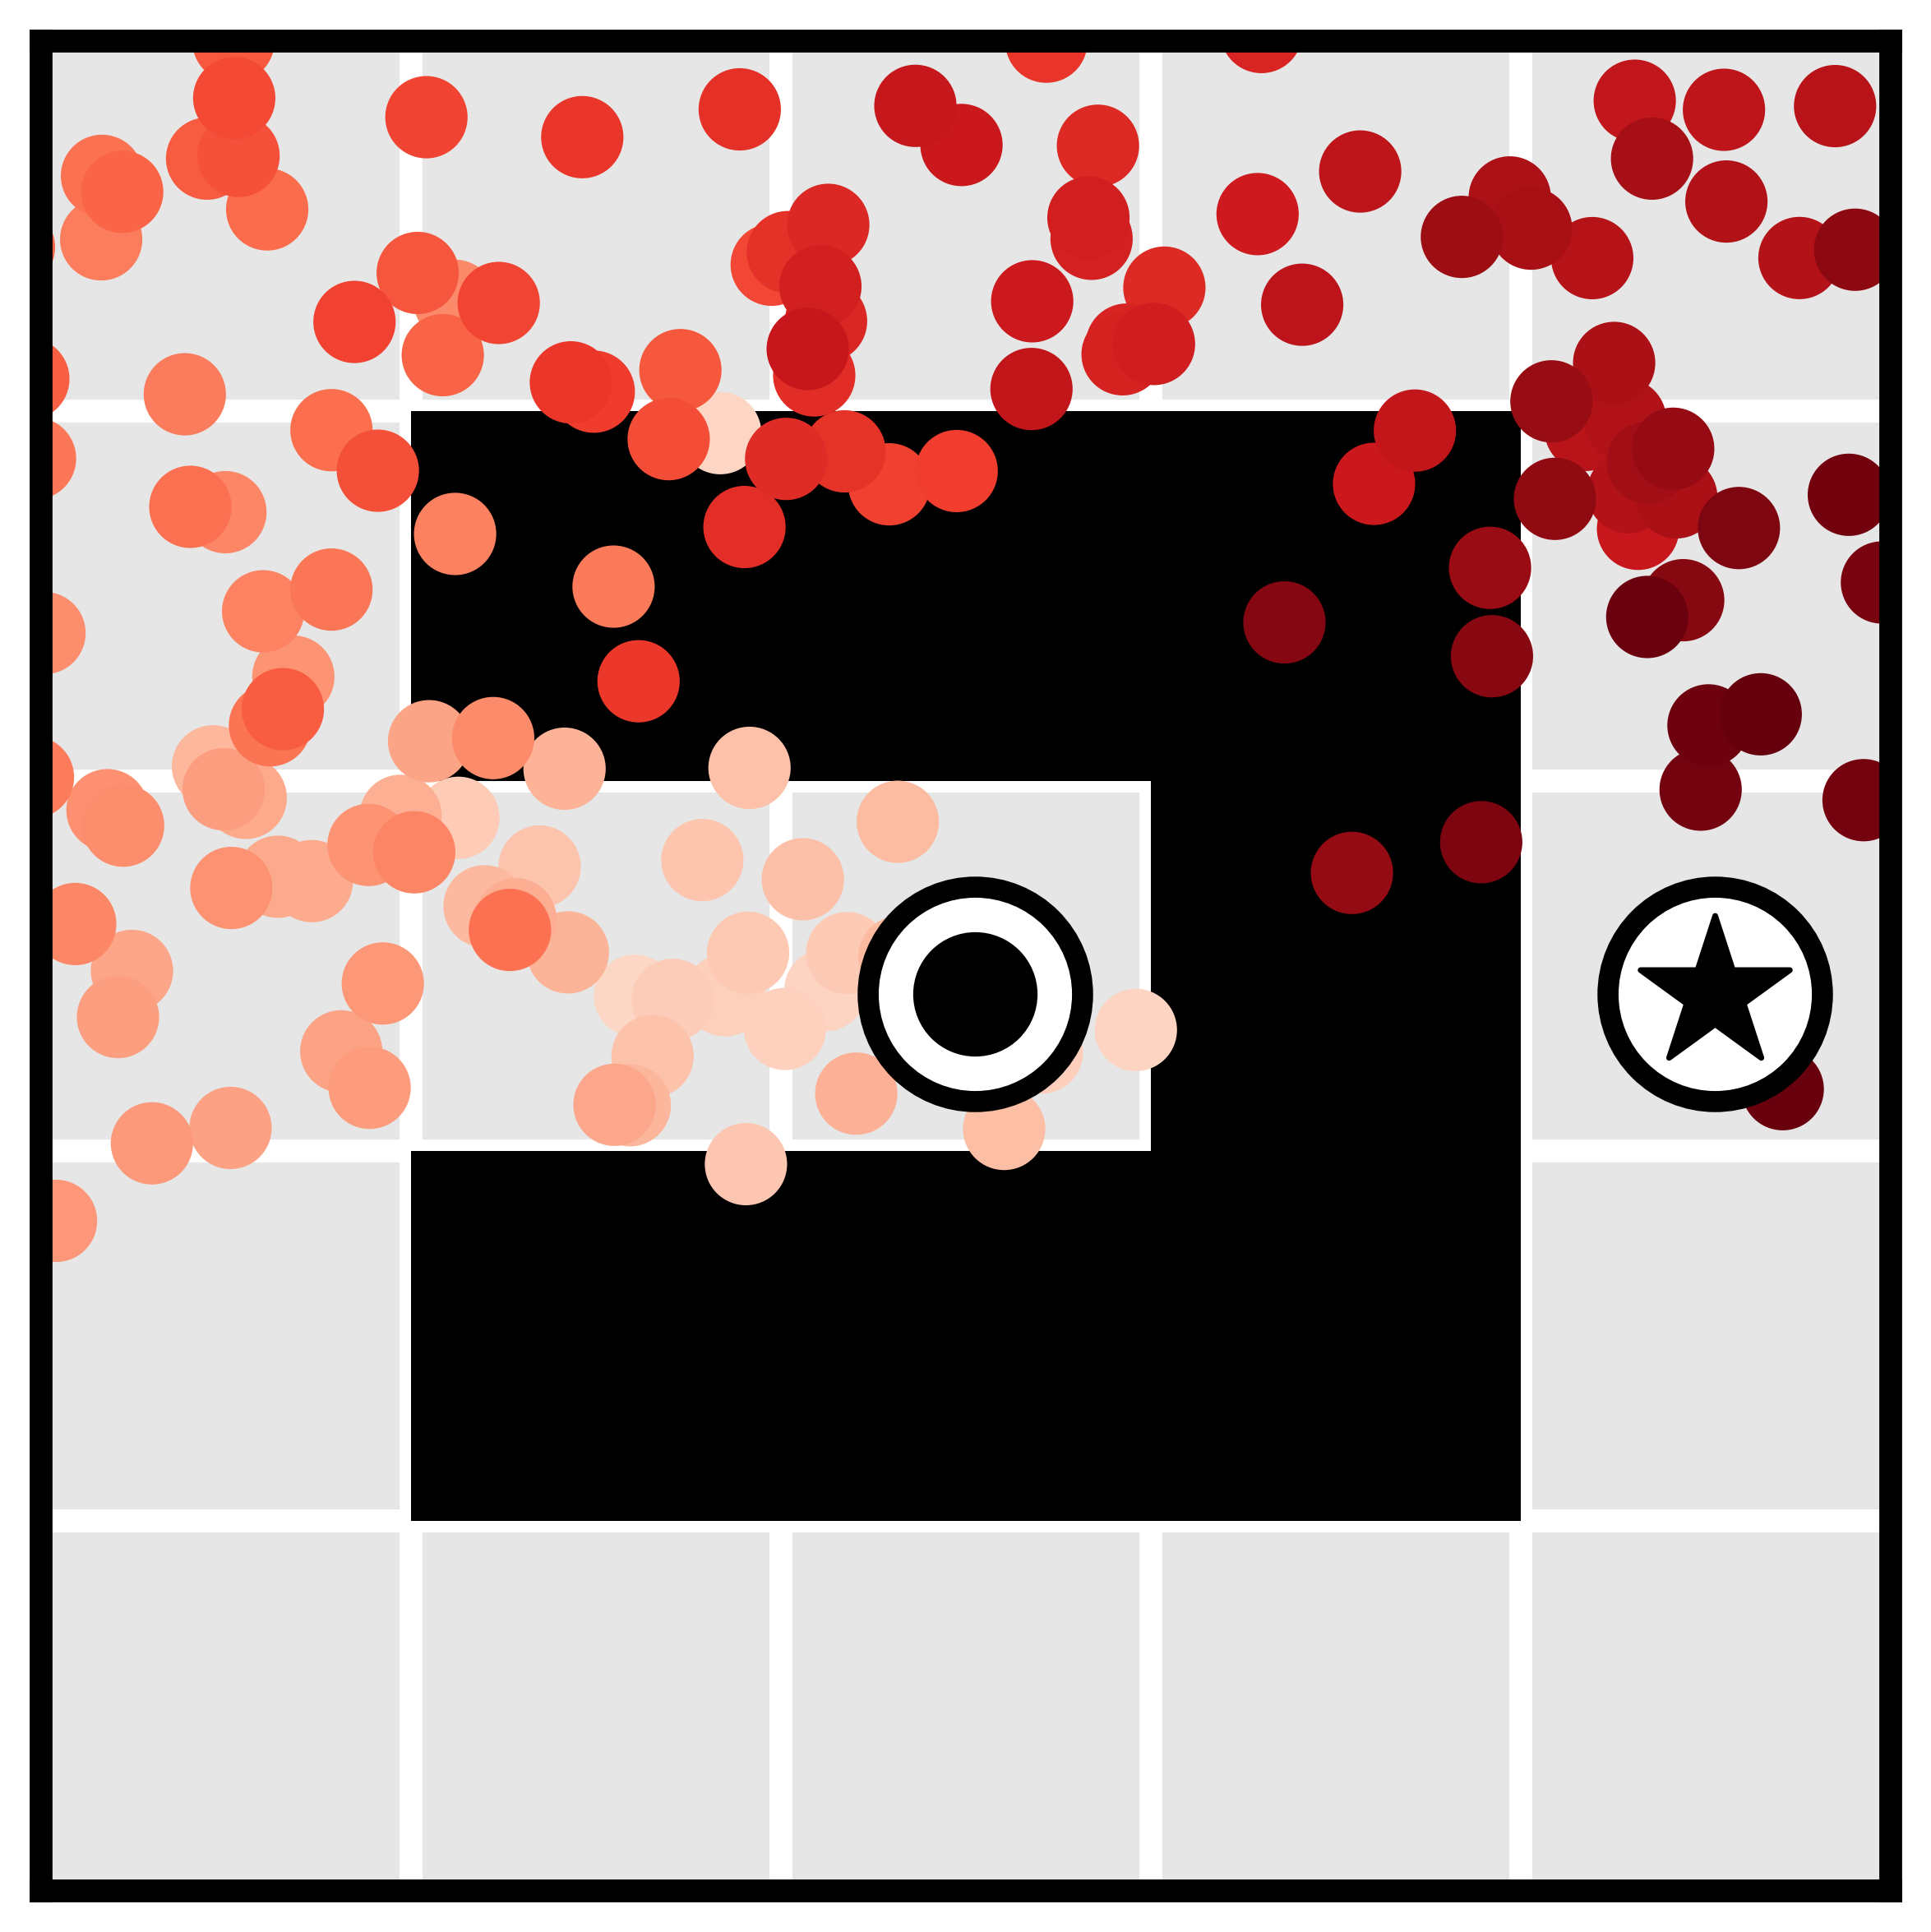
\includegraphics[width=2.5cm]{images/properties/planning_2.png}~
    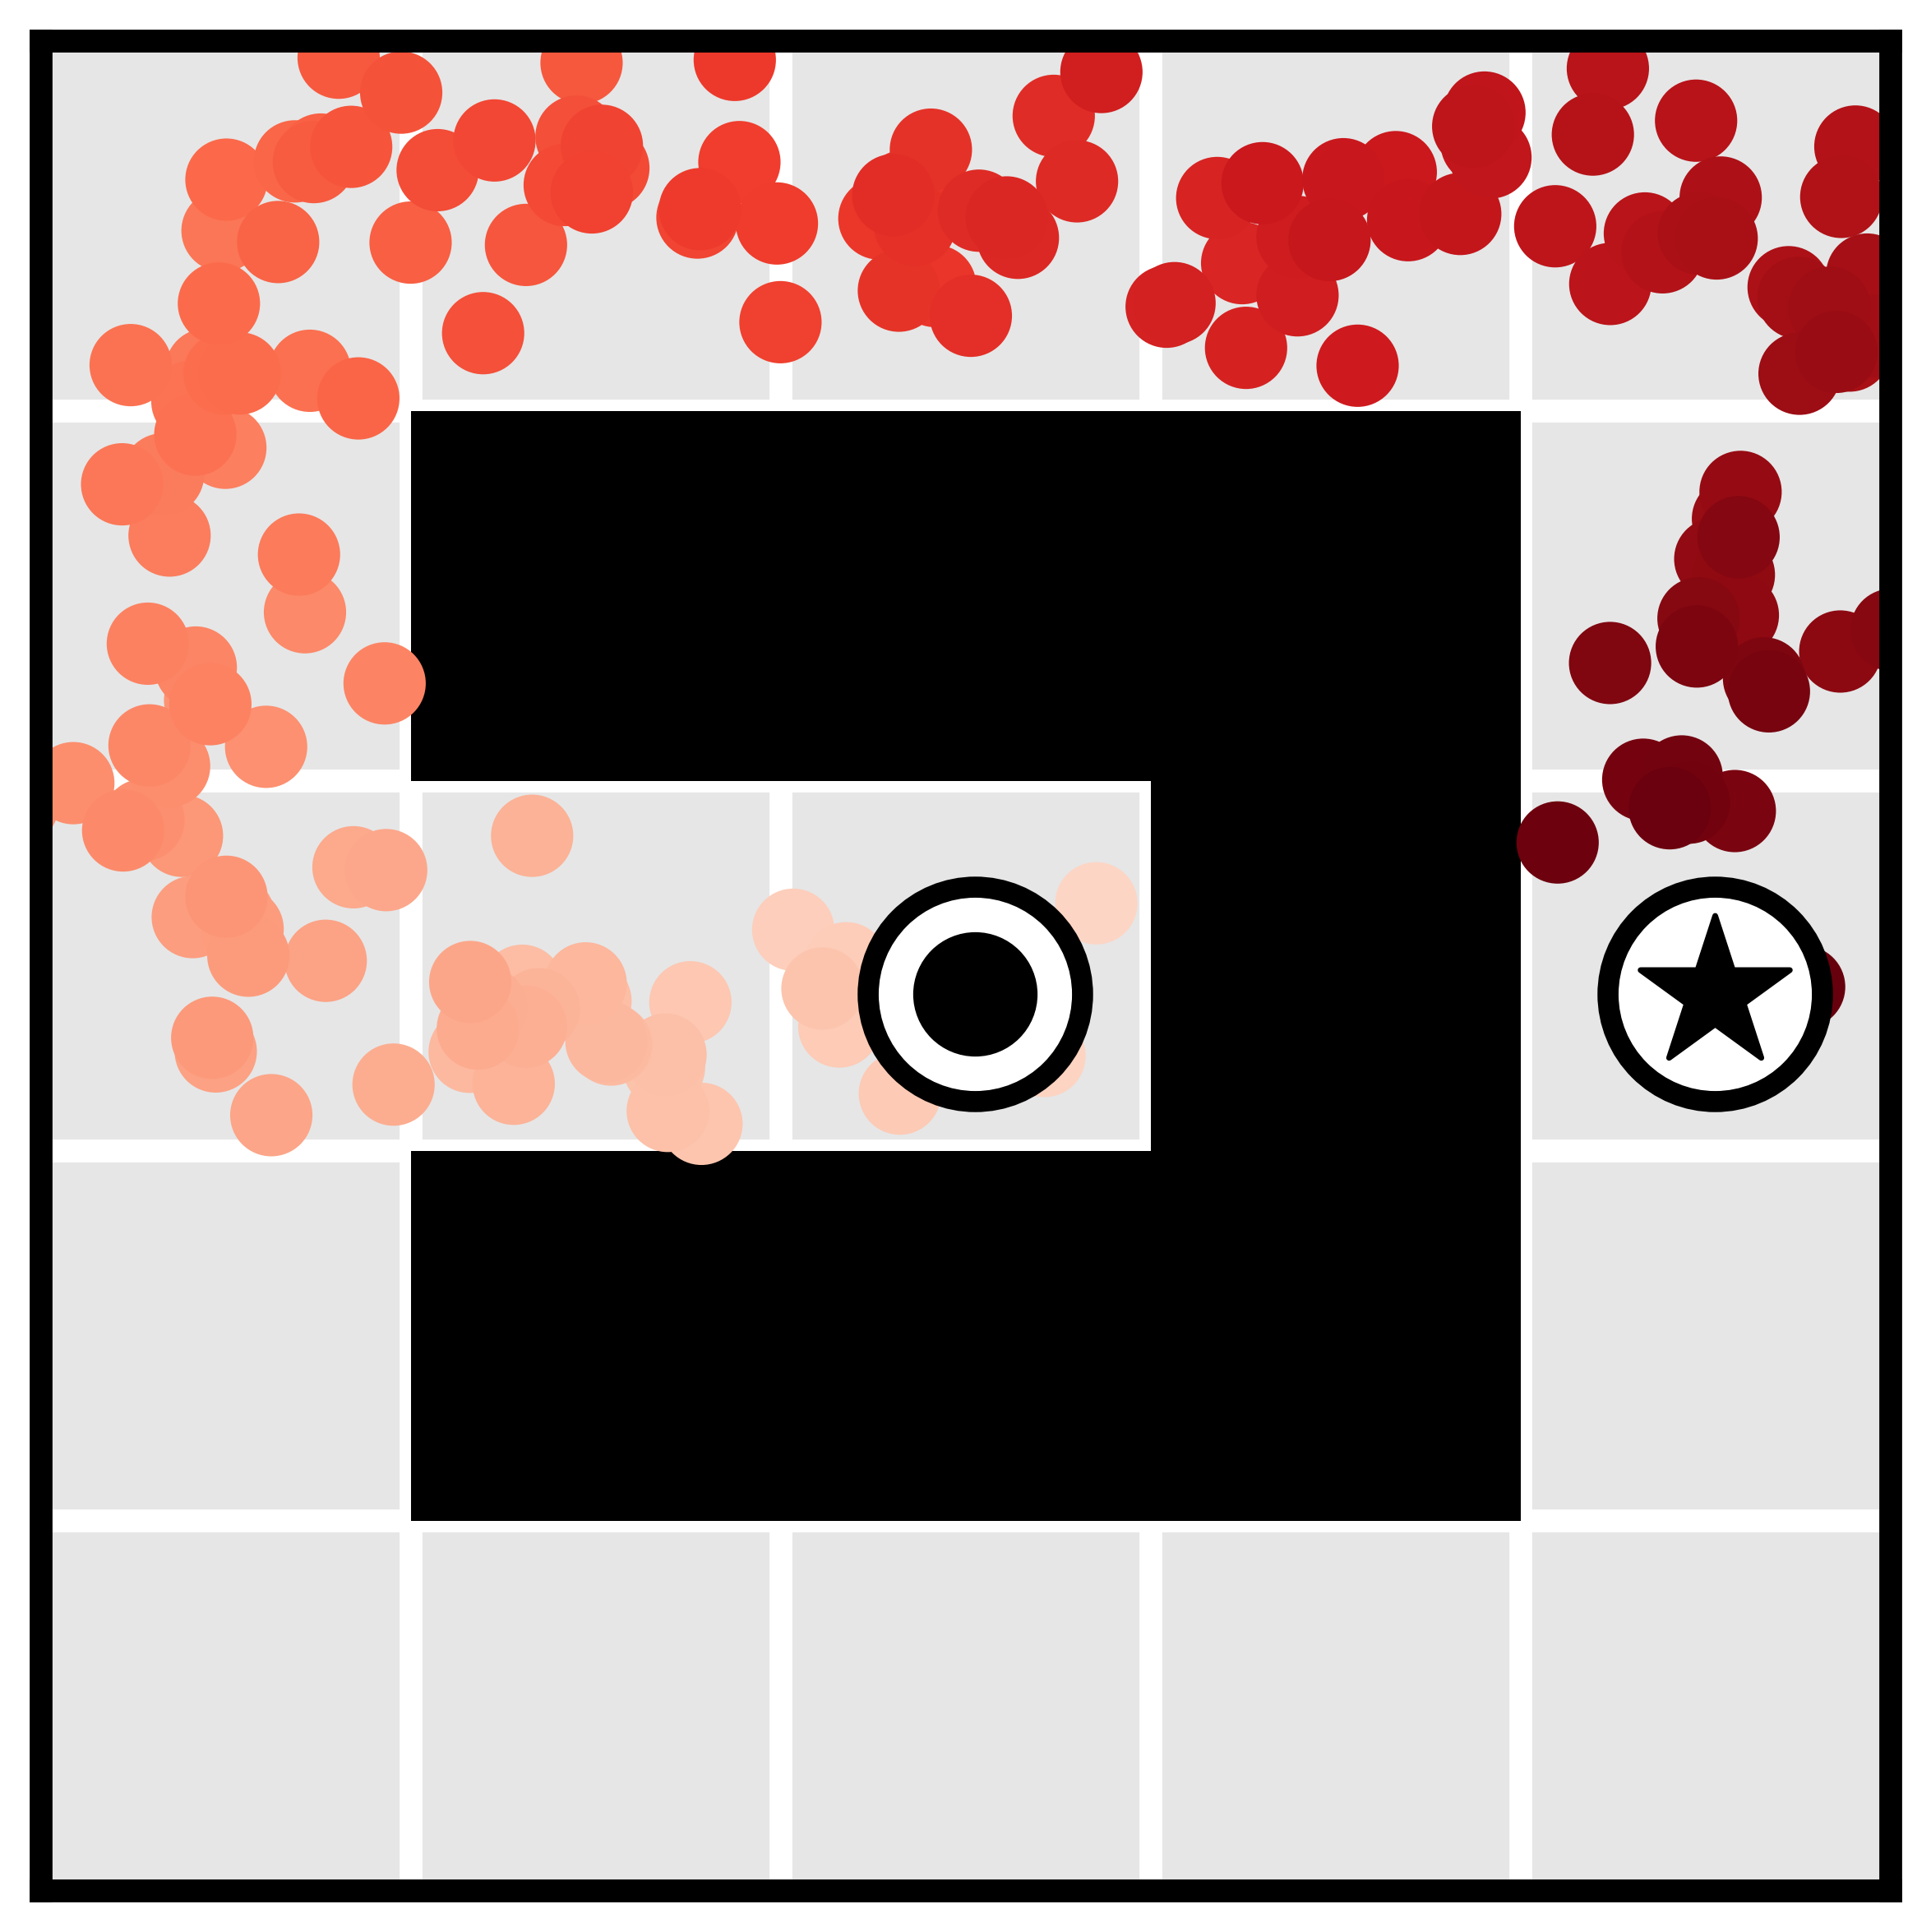
\includegraphics[width=2.5cm]{images/properties/planning_1.png}~
    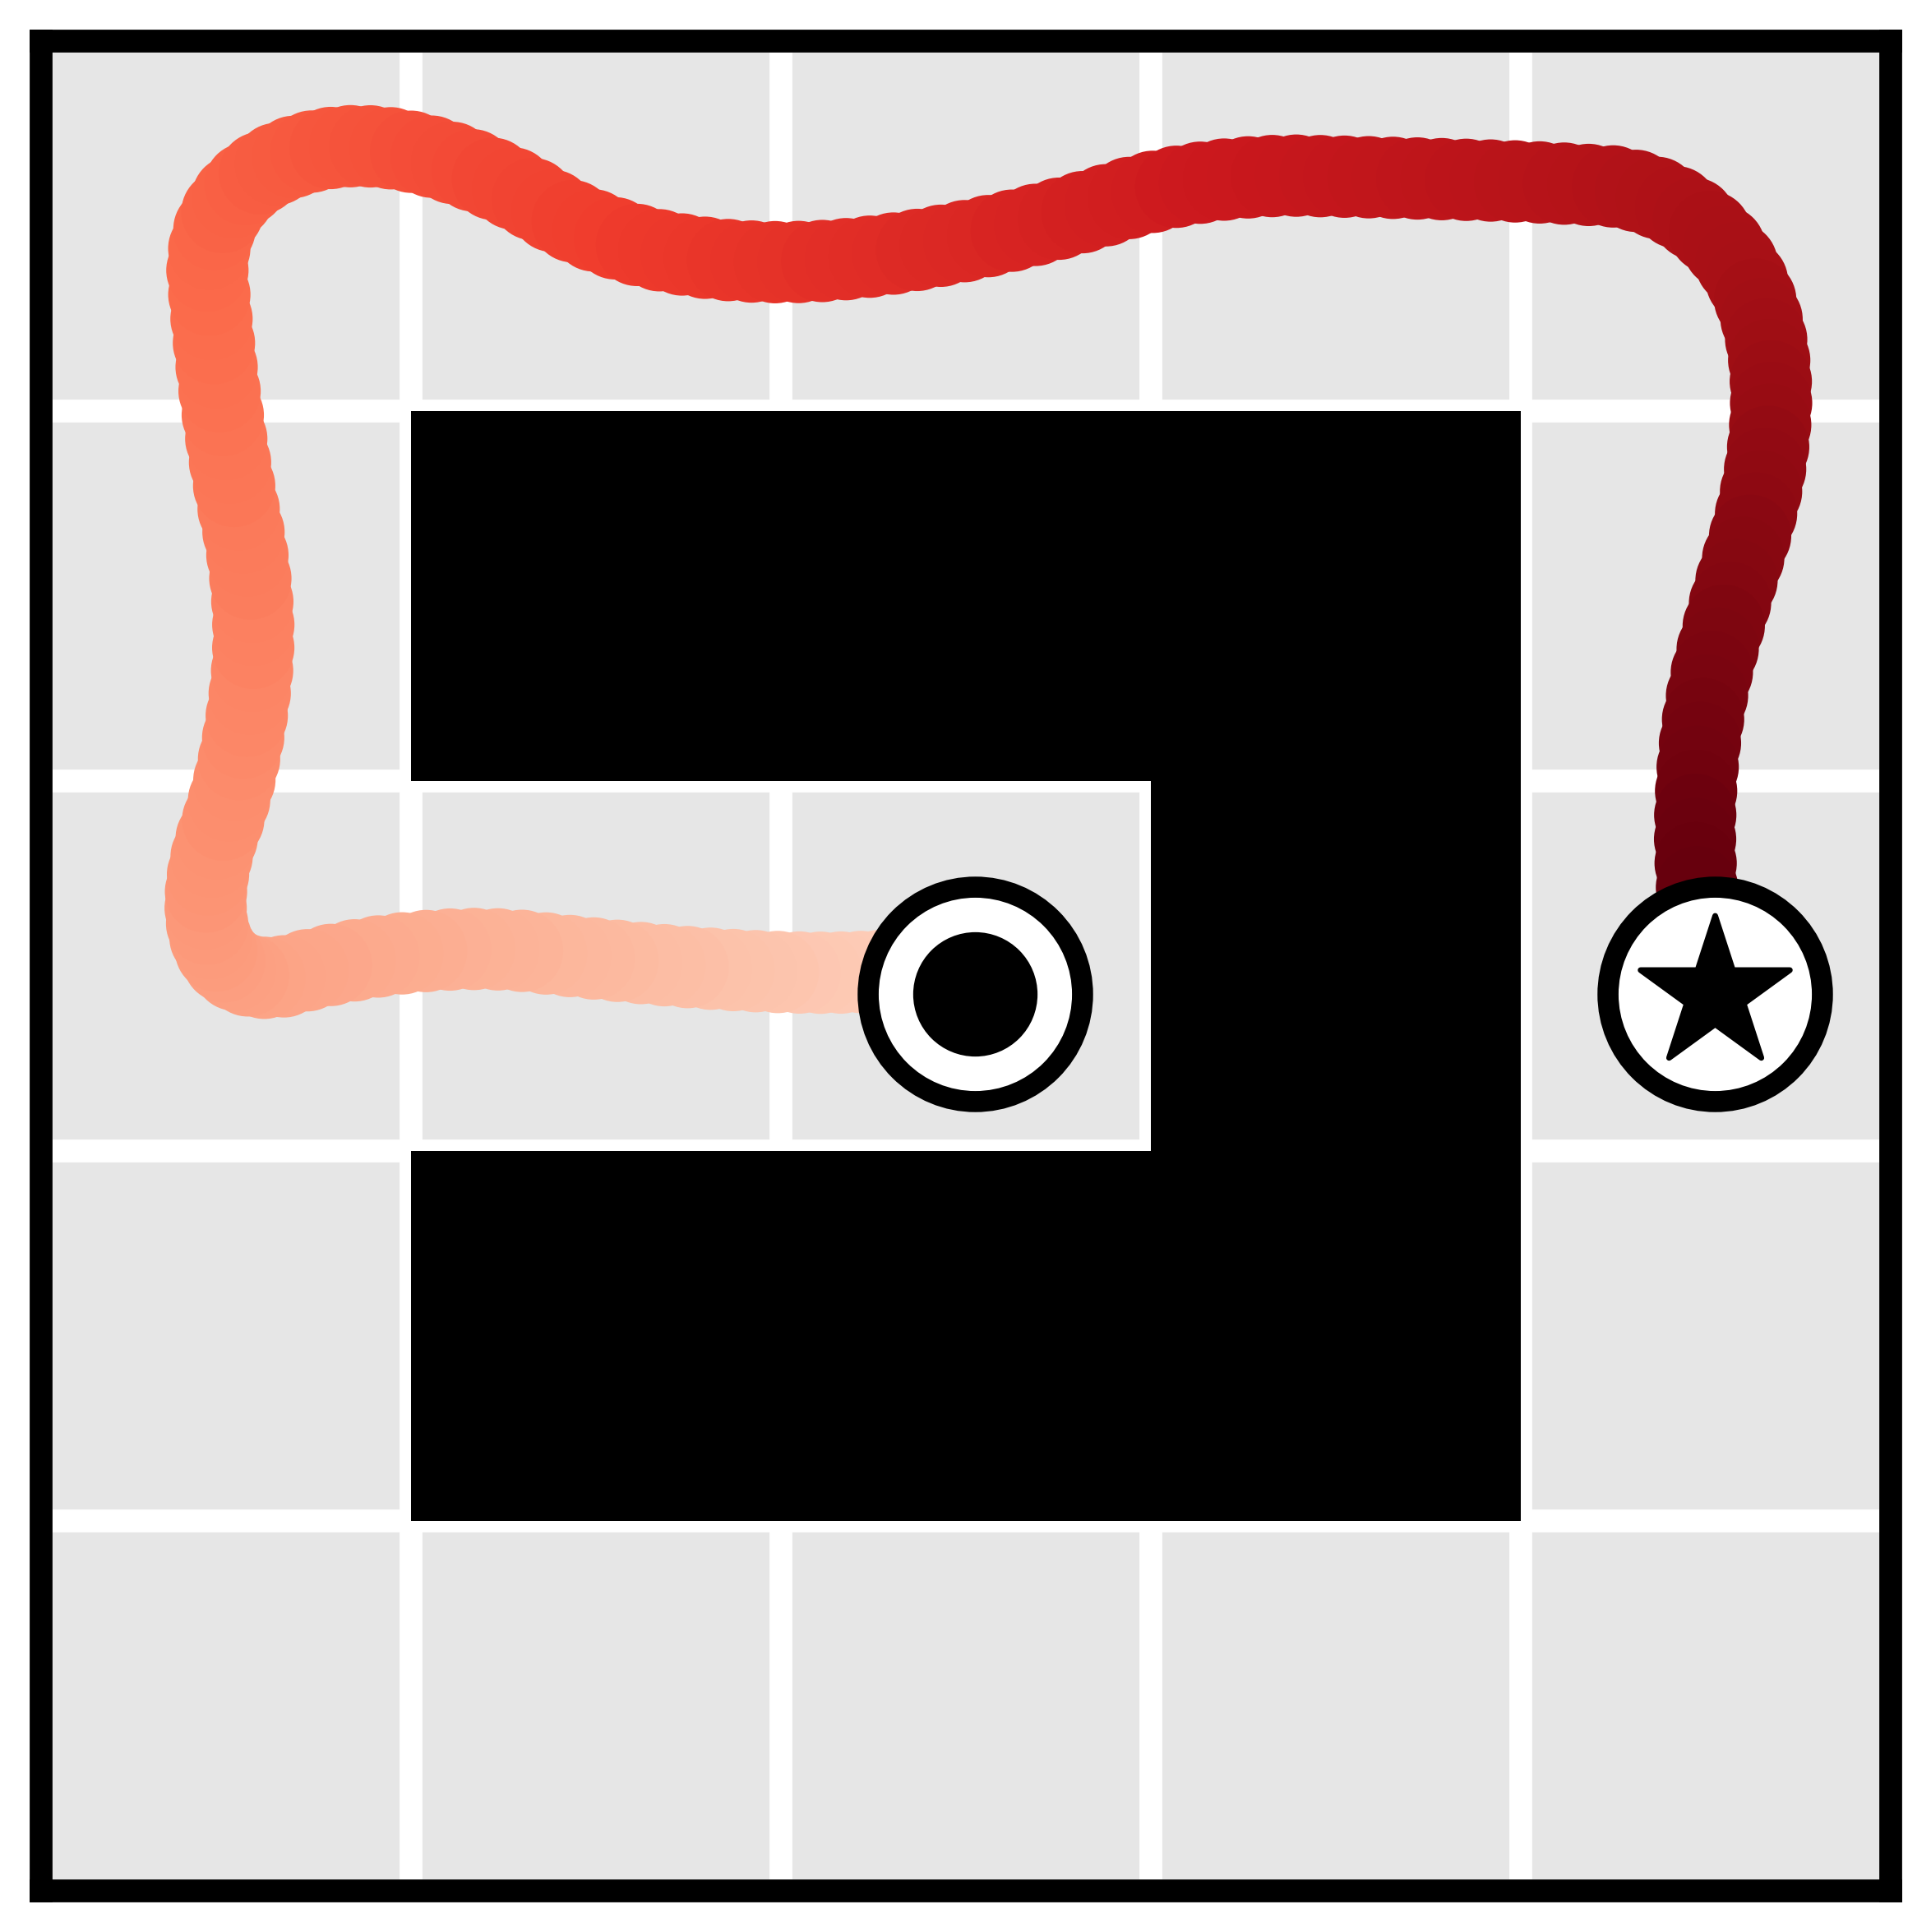
\includegraphics[width=2.5cm]{images/properties/planning_0.png} \\
    \vspace{-.4cm}
    \begin{center}
        \raisebox{.3\height}{denoising}~~
        \tikz \draw [-{Computer Modern Rightarrow[length=1.33mm, width=2mm]}, line width=.2mm] (0,0) -- (3,0); \\
    \end{center}
\end{minipage}%
%%%%
\begin{minipage}[t]{0.35\textwidth}
    \raisebox{2cm}{\textbf{b}}~~~
    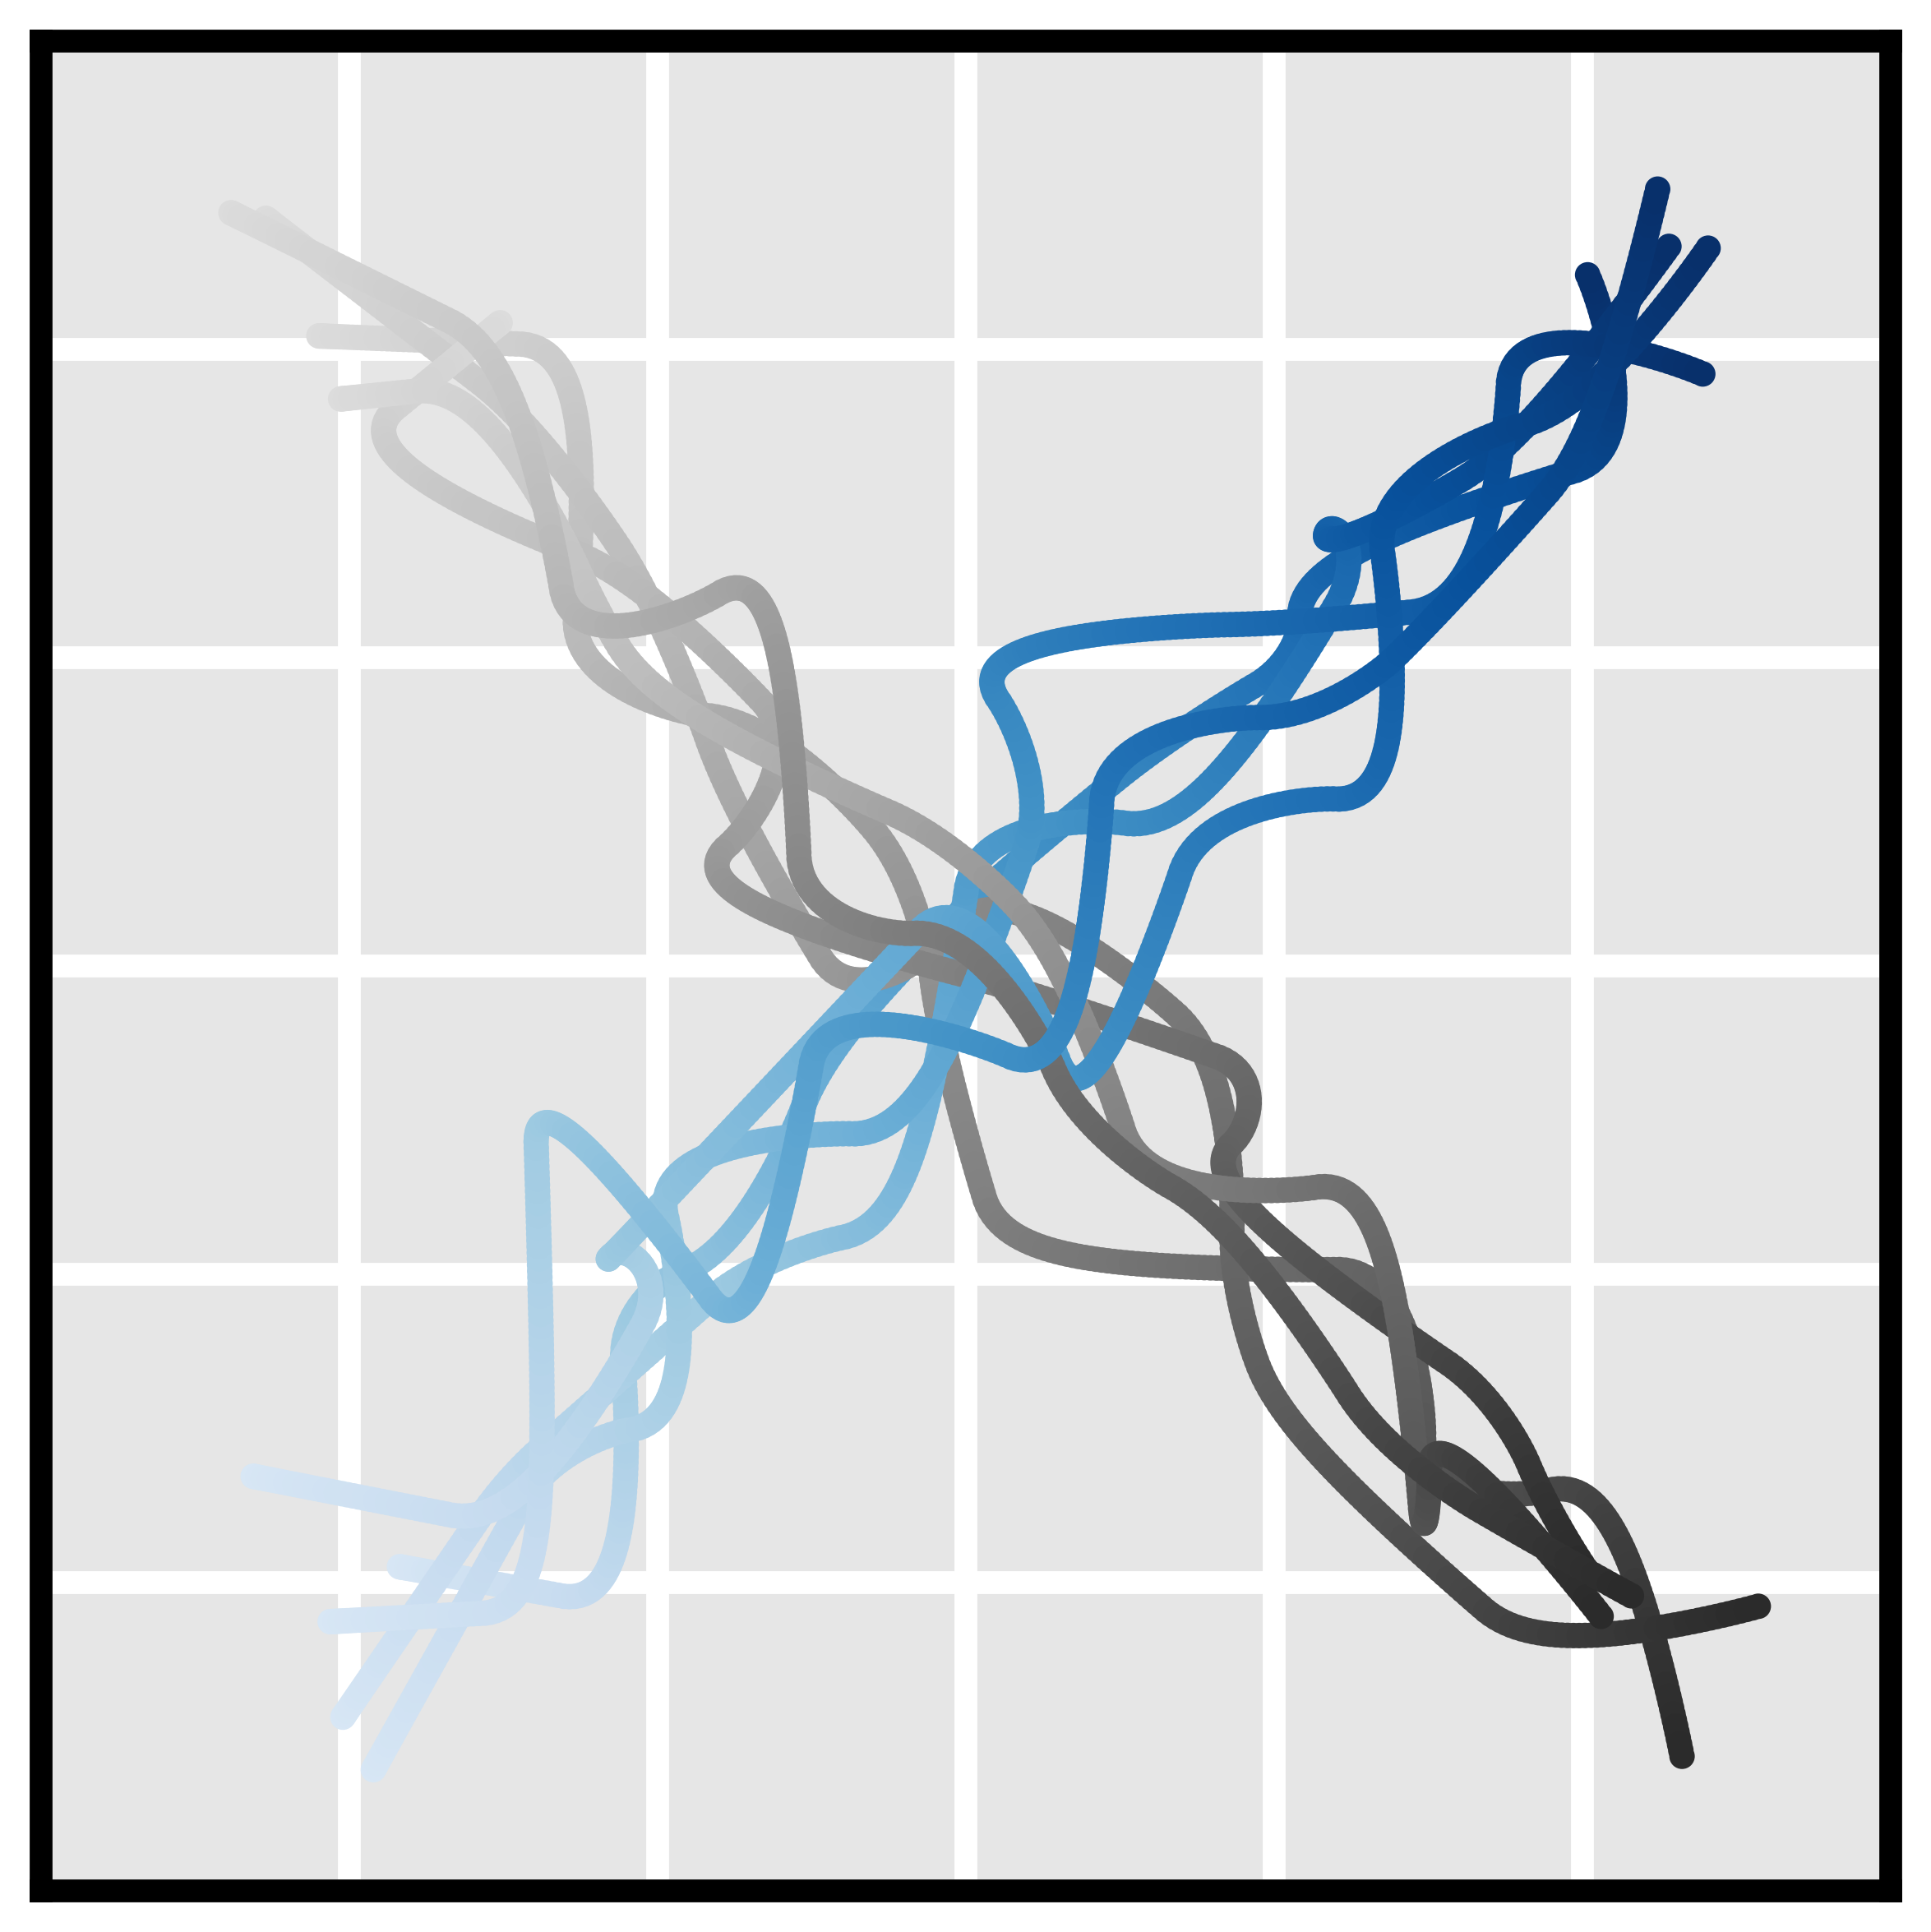
\includegraphics[width=2.5cm]{images/properties/stitching_data.png}~
    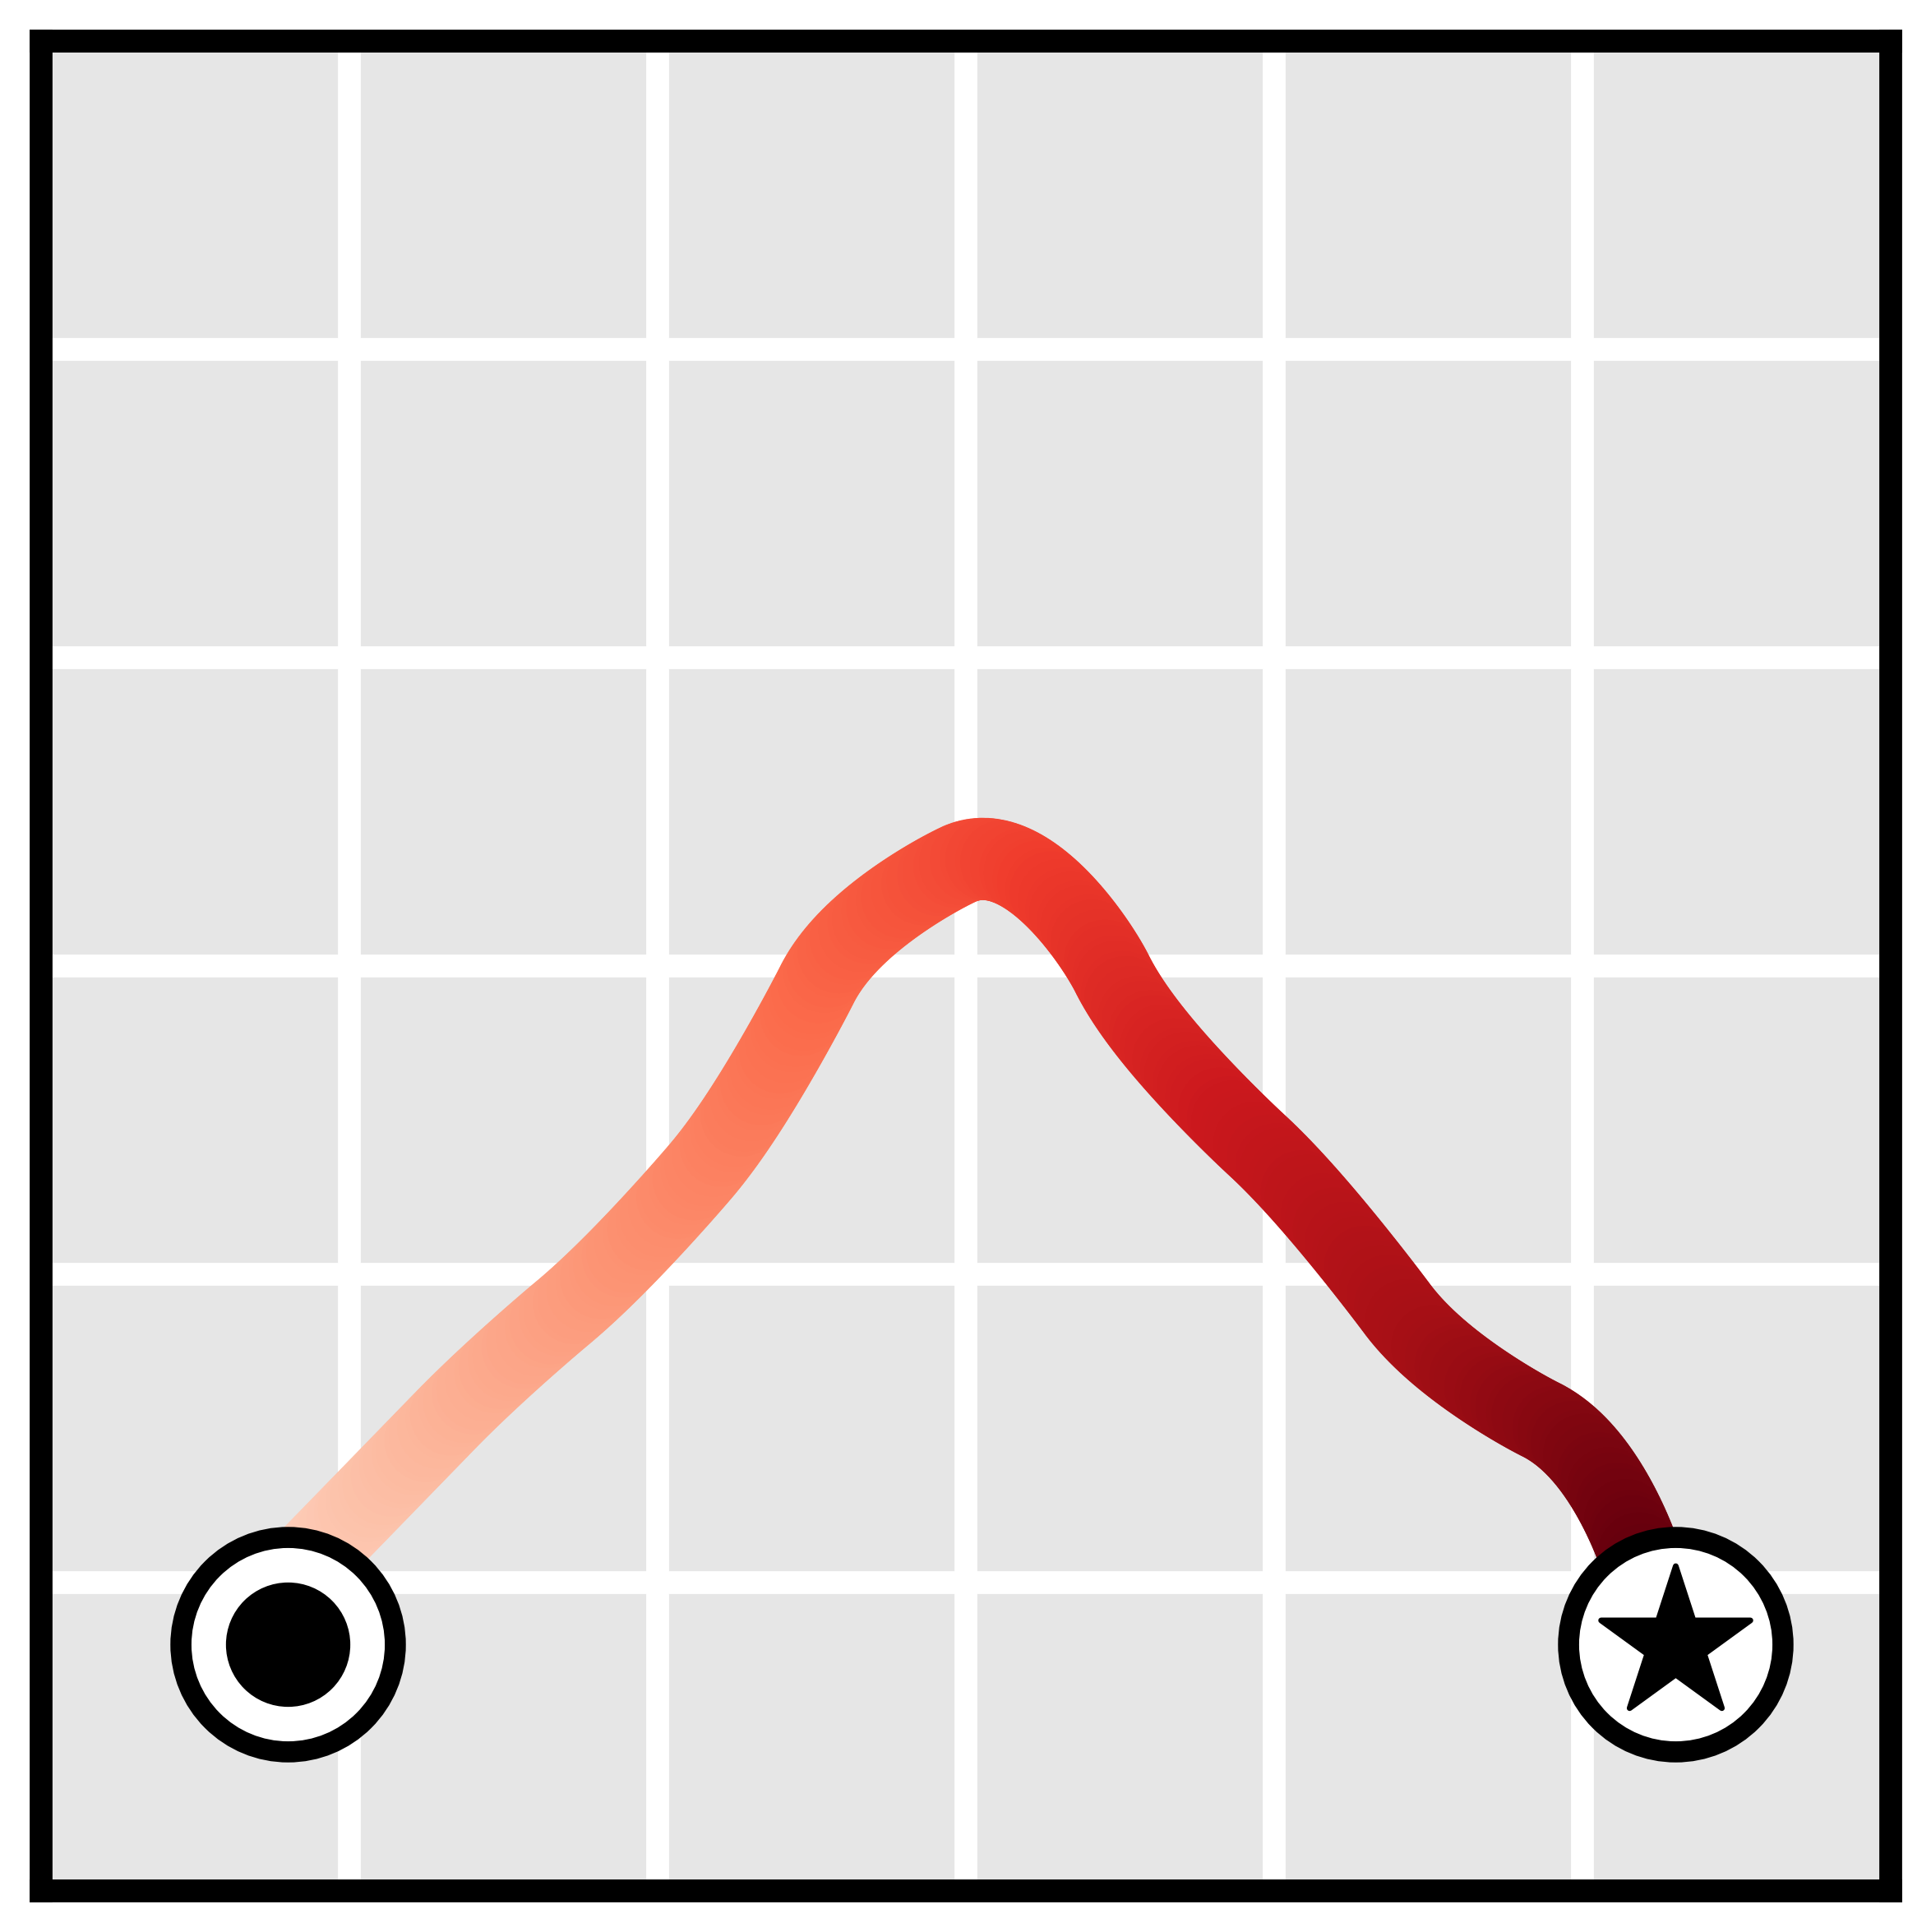
\includegraphics[width=2.5cm]{images/properties/stitching_plan.png} \\
    \vspace{-.5cm}
    \begin{center}
            \hspace{0.1cm} data \hspace{1.8cm} plan \\
    \end{center}
\end{minipage} \\
\vspace{.4cm}
%%%%
\begin{minipage}[t]{0.55\textwidth}
    \raisebox{2cm}{\textbf{c}}~~~
    \raisebox{0.3cm}{\undersetimage{images/properties/rand_0.png}{$\btau{N}$}{-0.25}}
        \raisebox{1.2cm}{$\rightarrow$}
        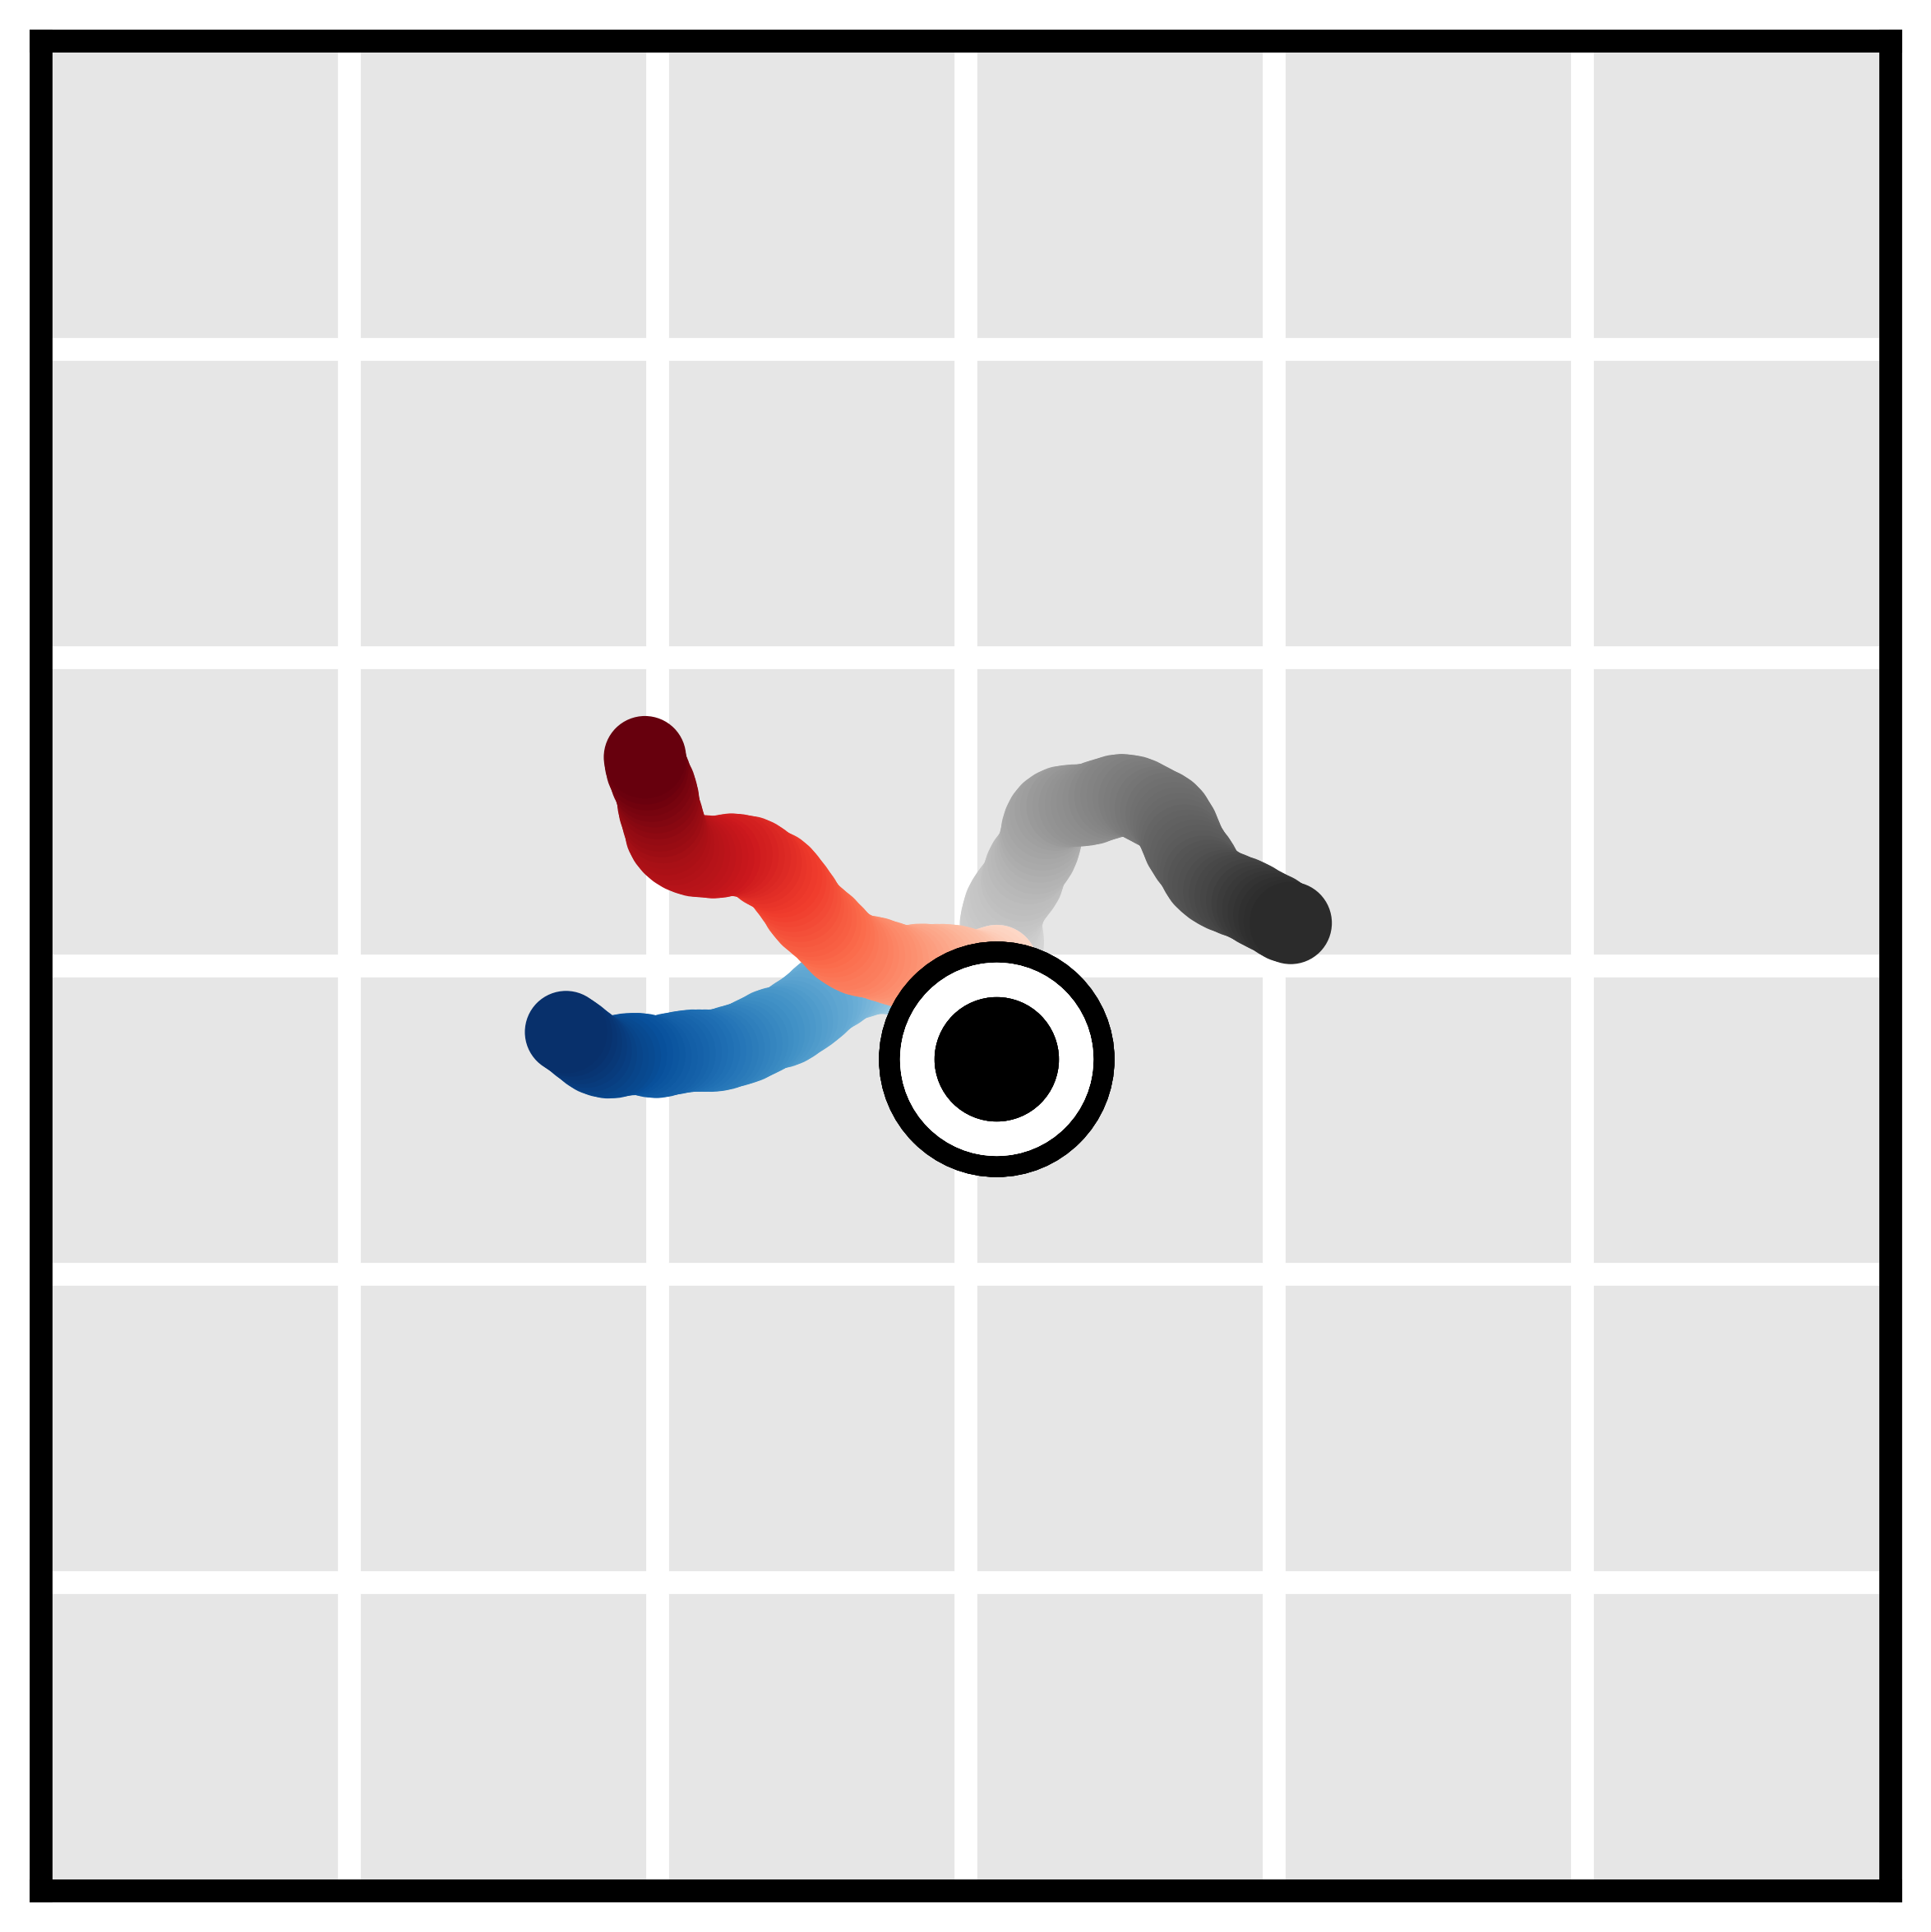
\includegraphics[width=2.5cm]{images/properties/variable_0.png}
        ~~
    \raisebox{-0.1cm}{\undersetimage{images/properties/rand_1.png}{$\btau{N}$}{-0.15}}
        \raisebox{1.2cm}{$\rightarrow$}
        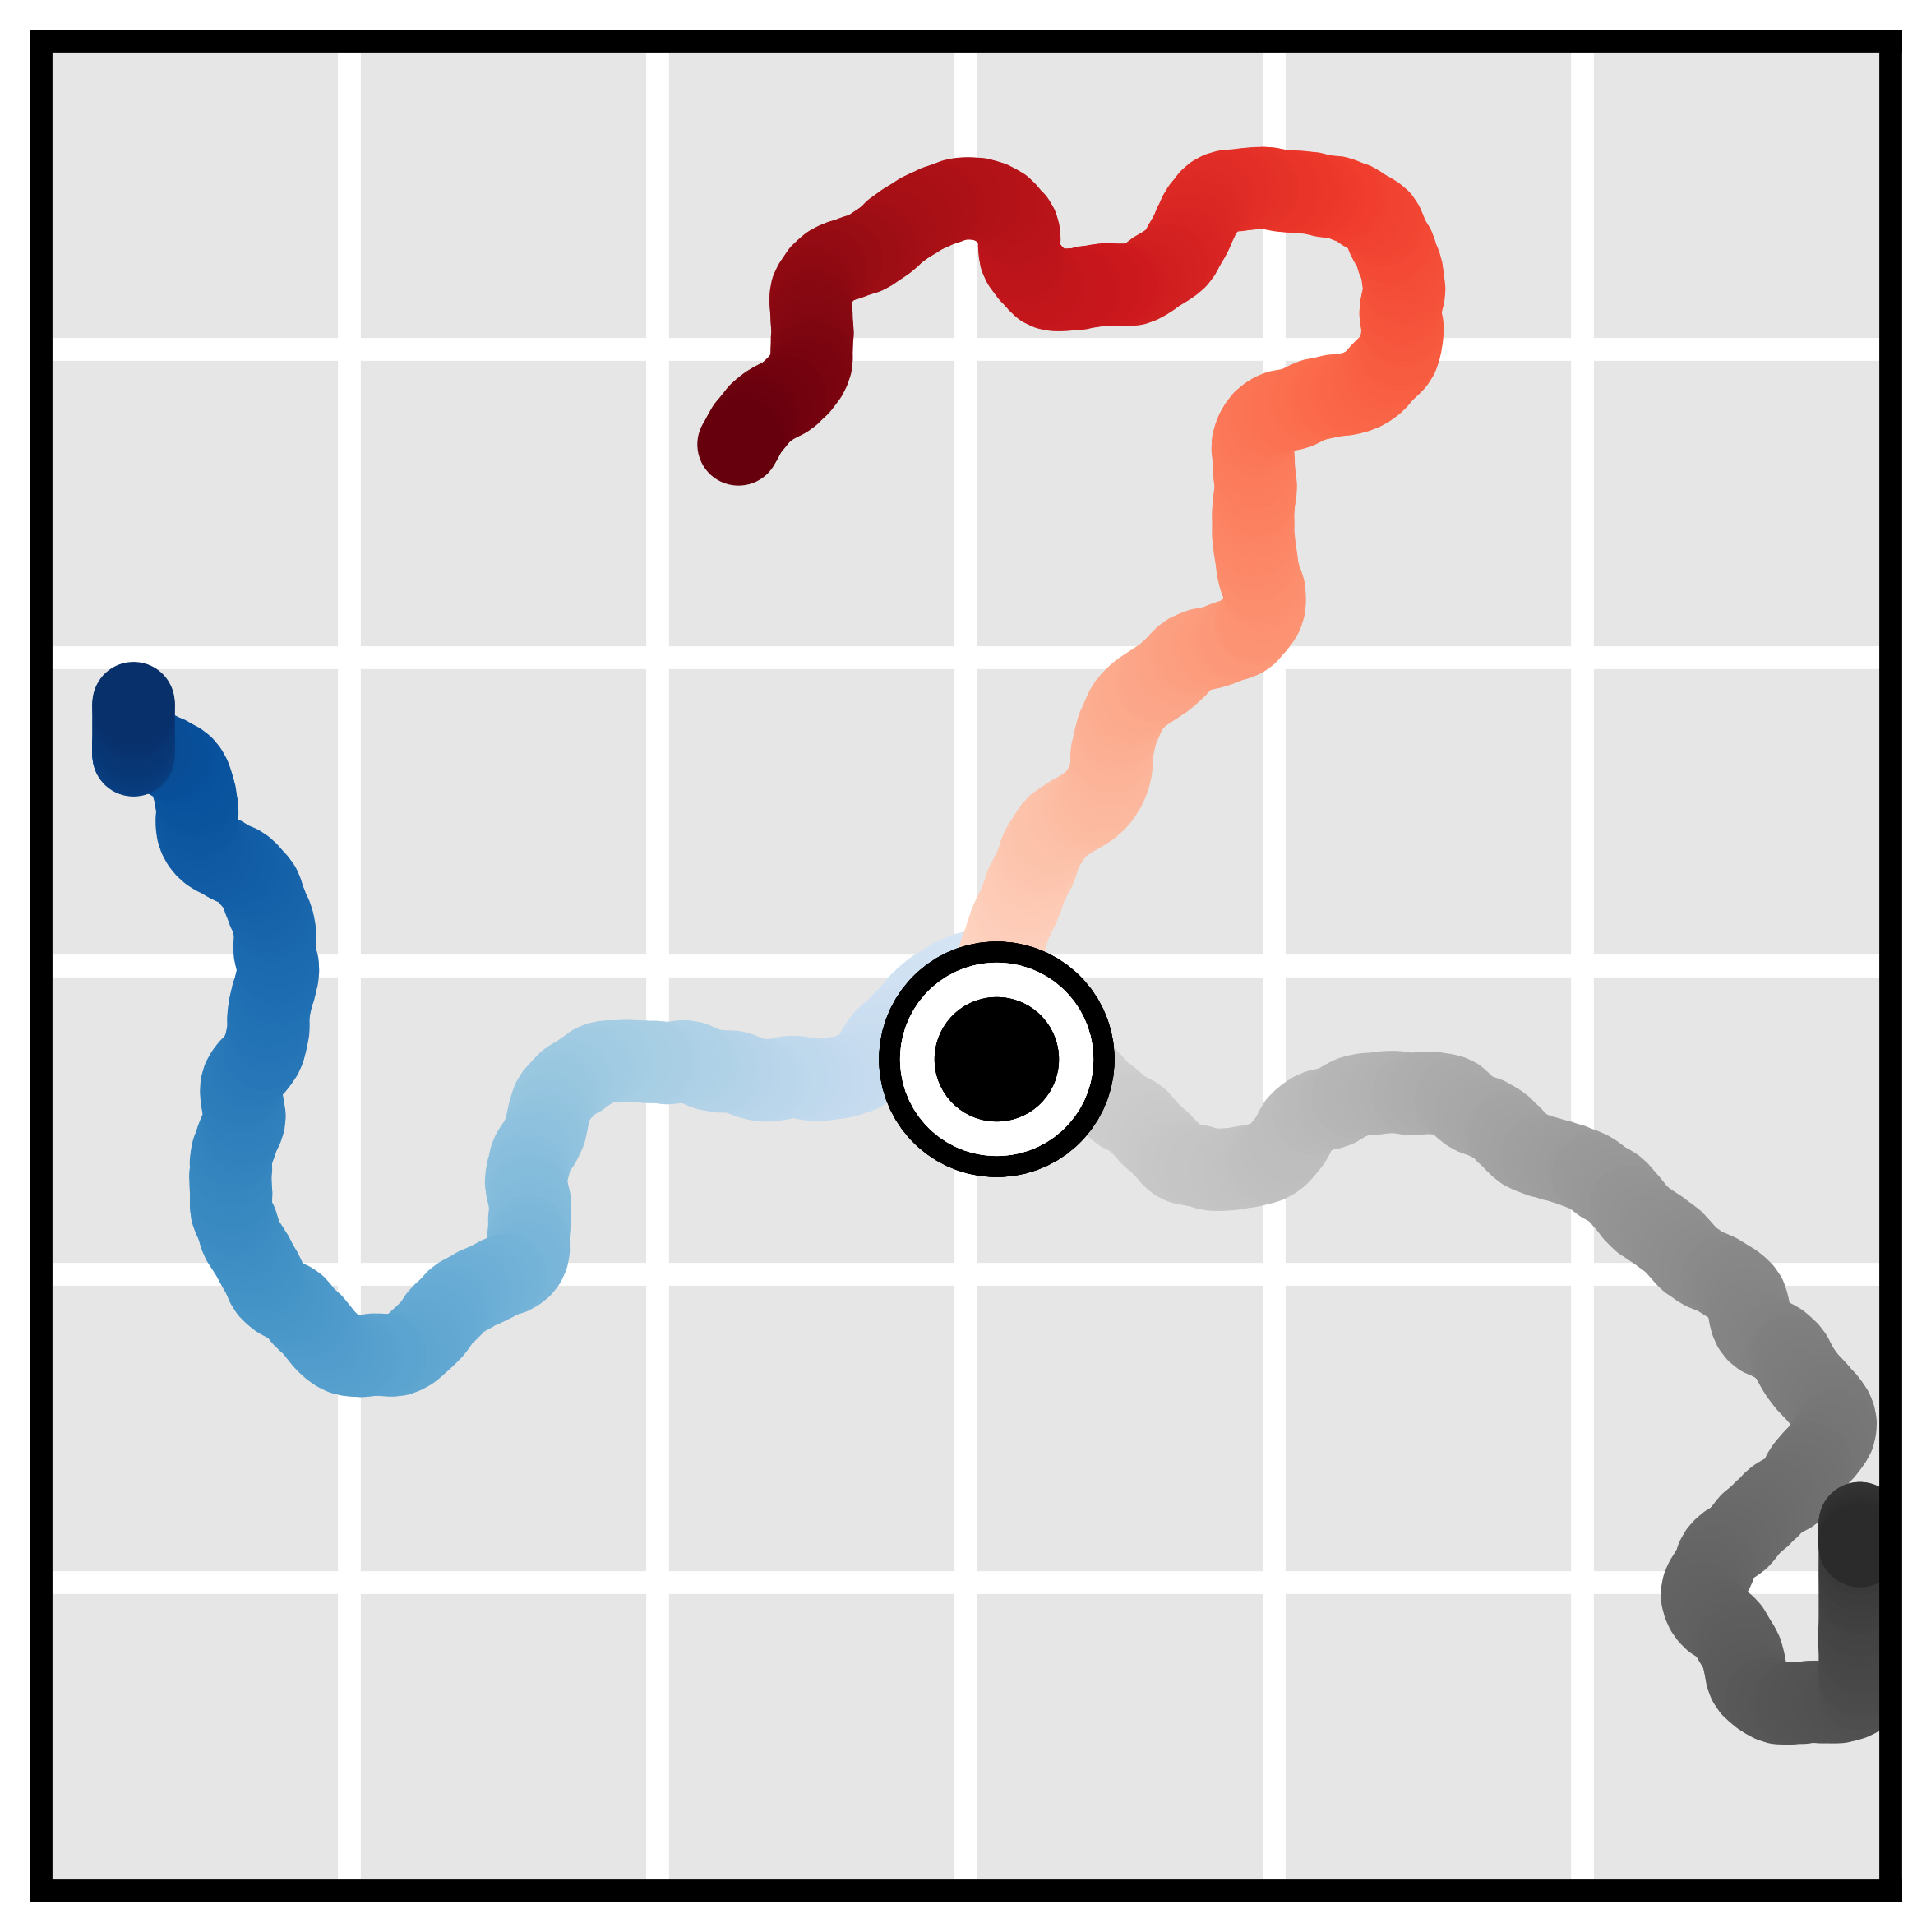
\includegraphics[width=2.5cm]{images/properties/variable_1_3.png} \\
    % ~~~~\raisebox{2cm}{$\btau{N}$} \\
\end{minipage}%
%%%%
\begin{minipage}[t]{0.35\textwidth}
    \raisebox{2cm}{\textbf{d}}~~~
    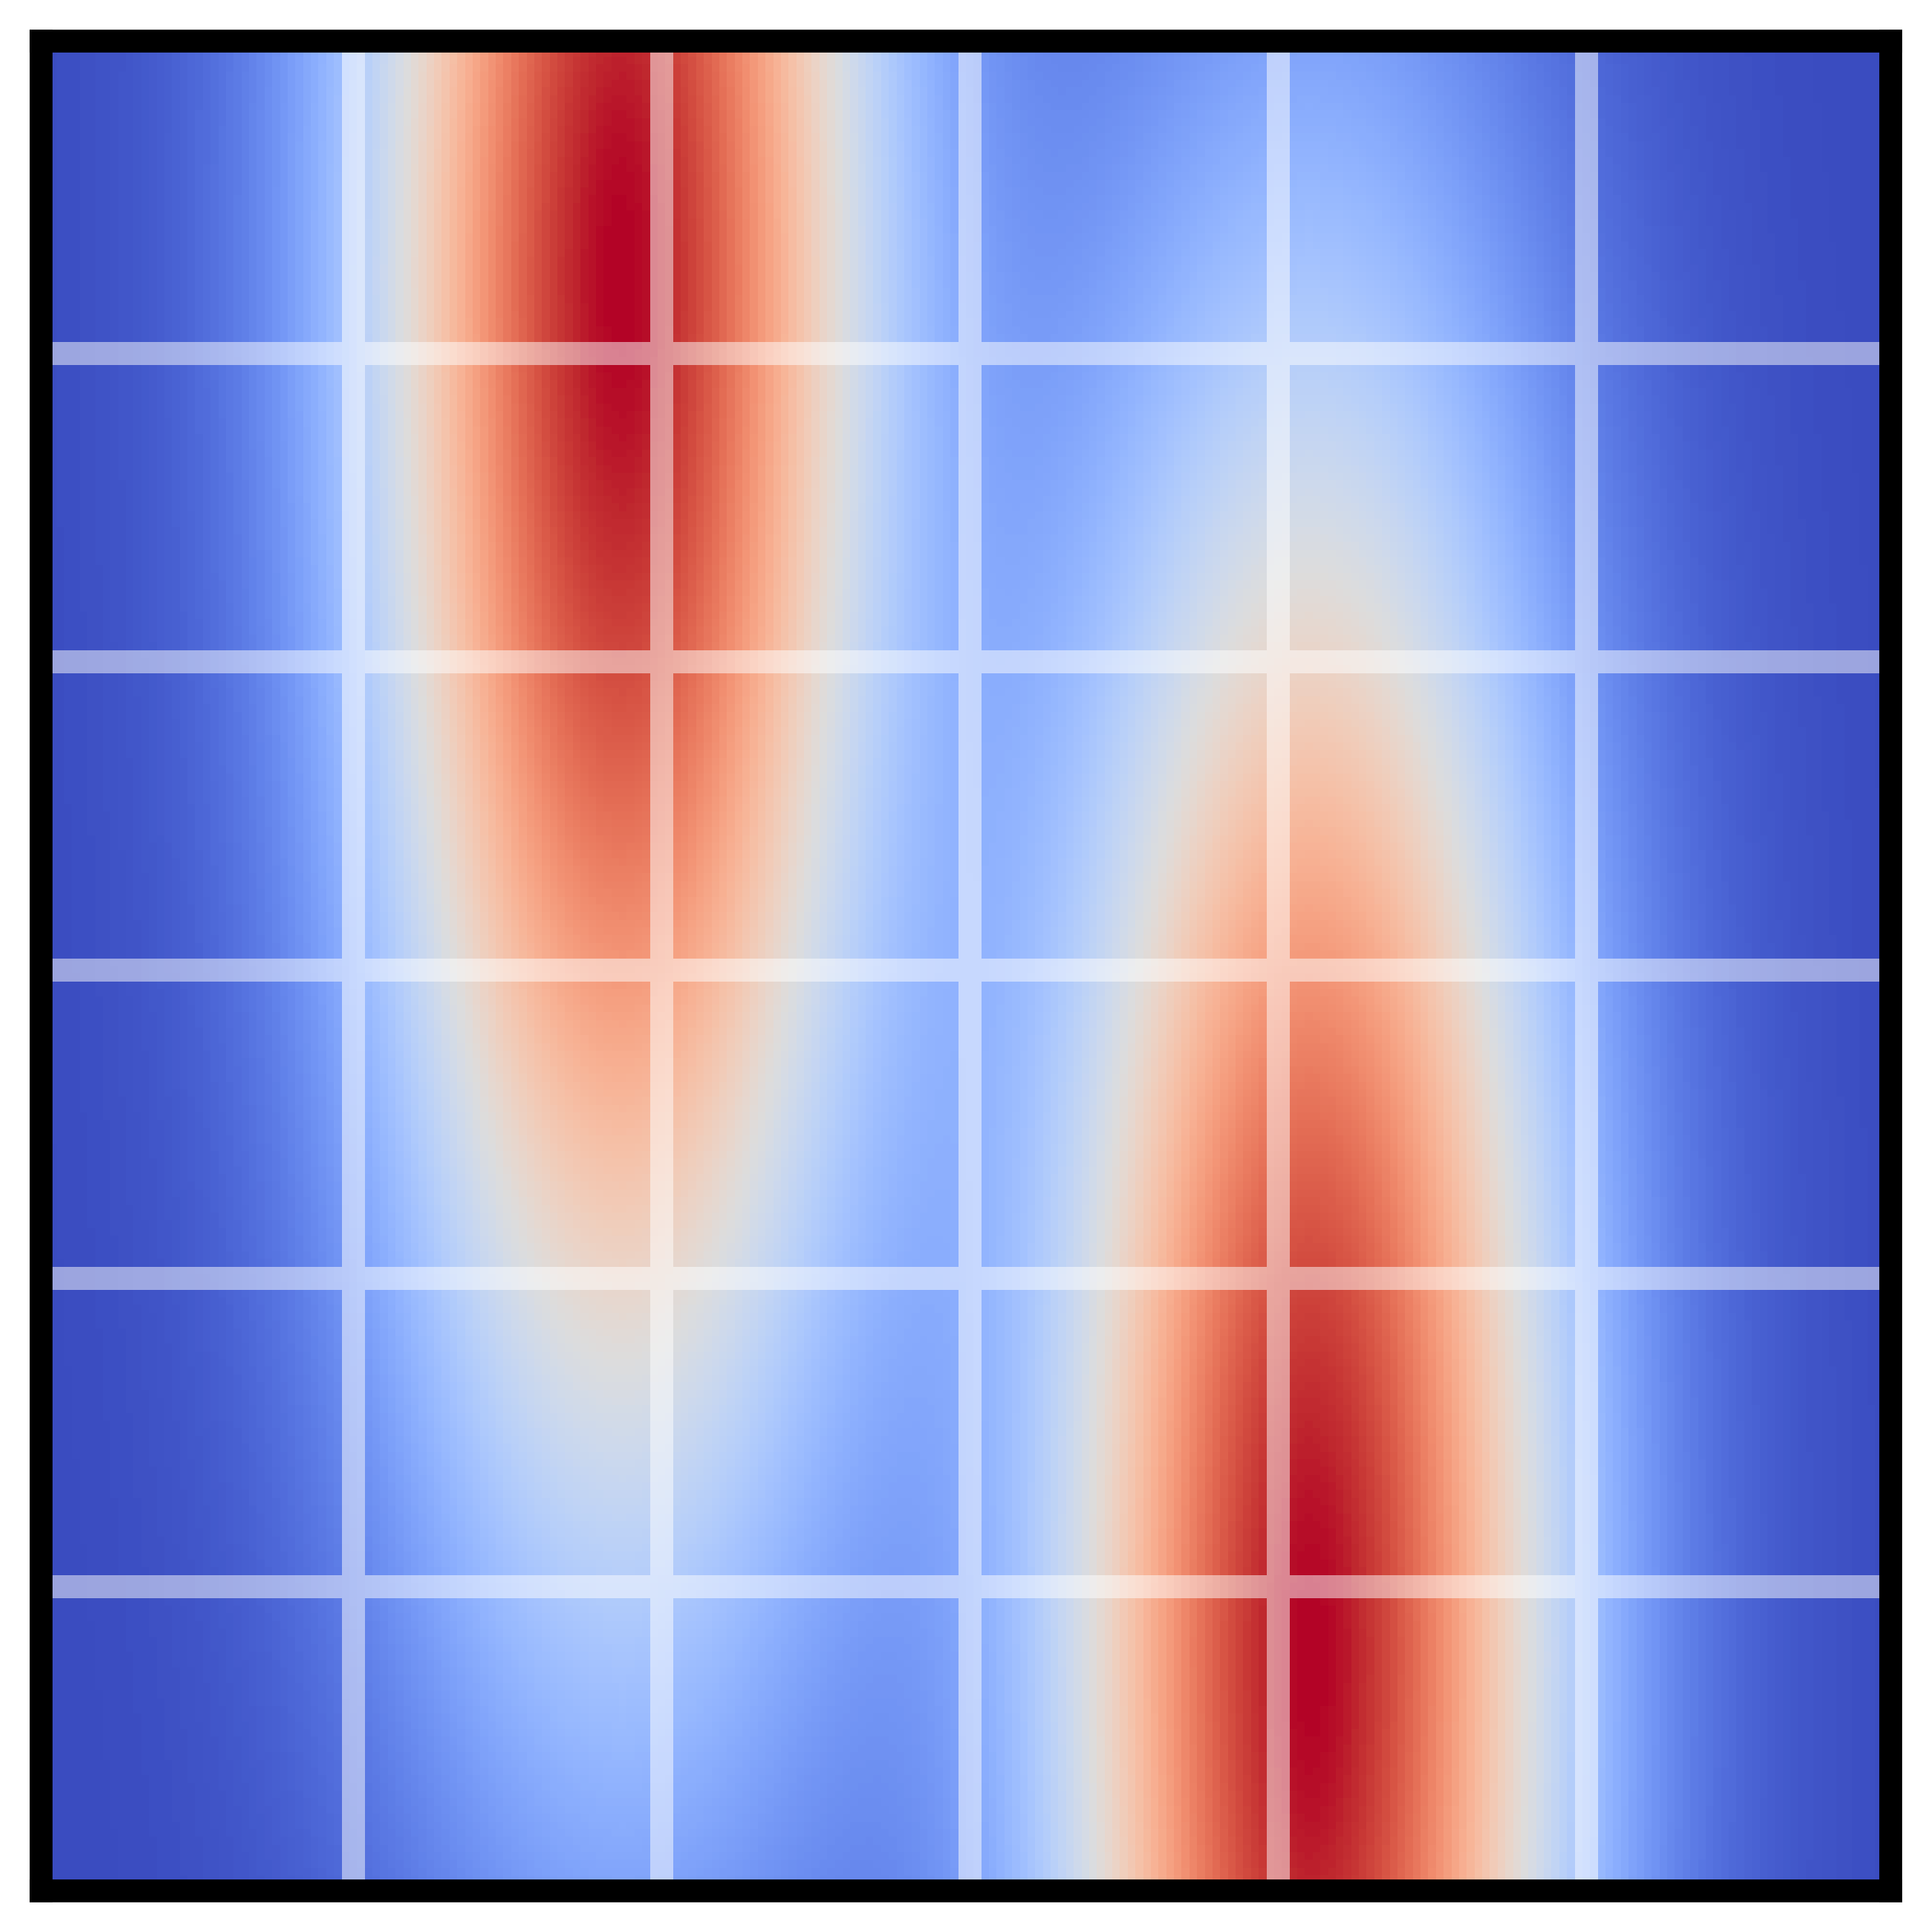
\includegraphics[width=2.5cm]{images/properties/reward.png}~
    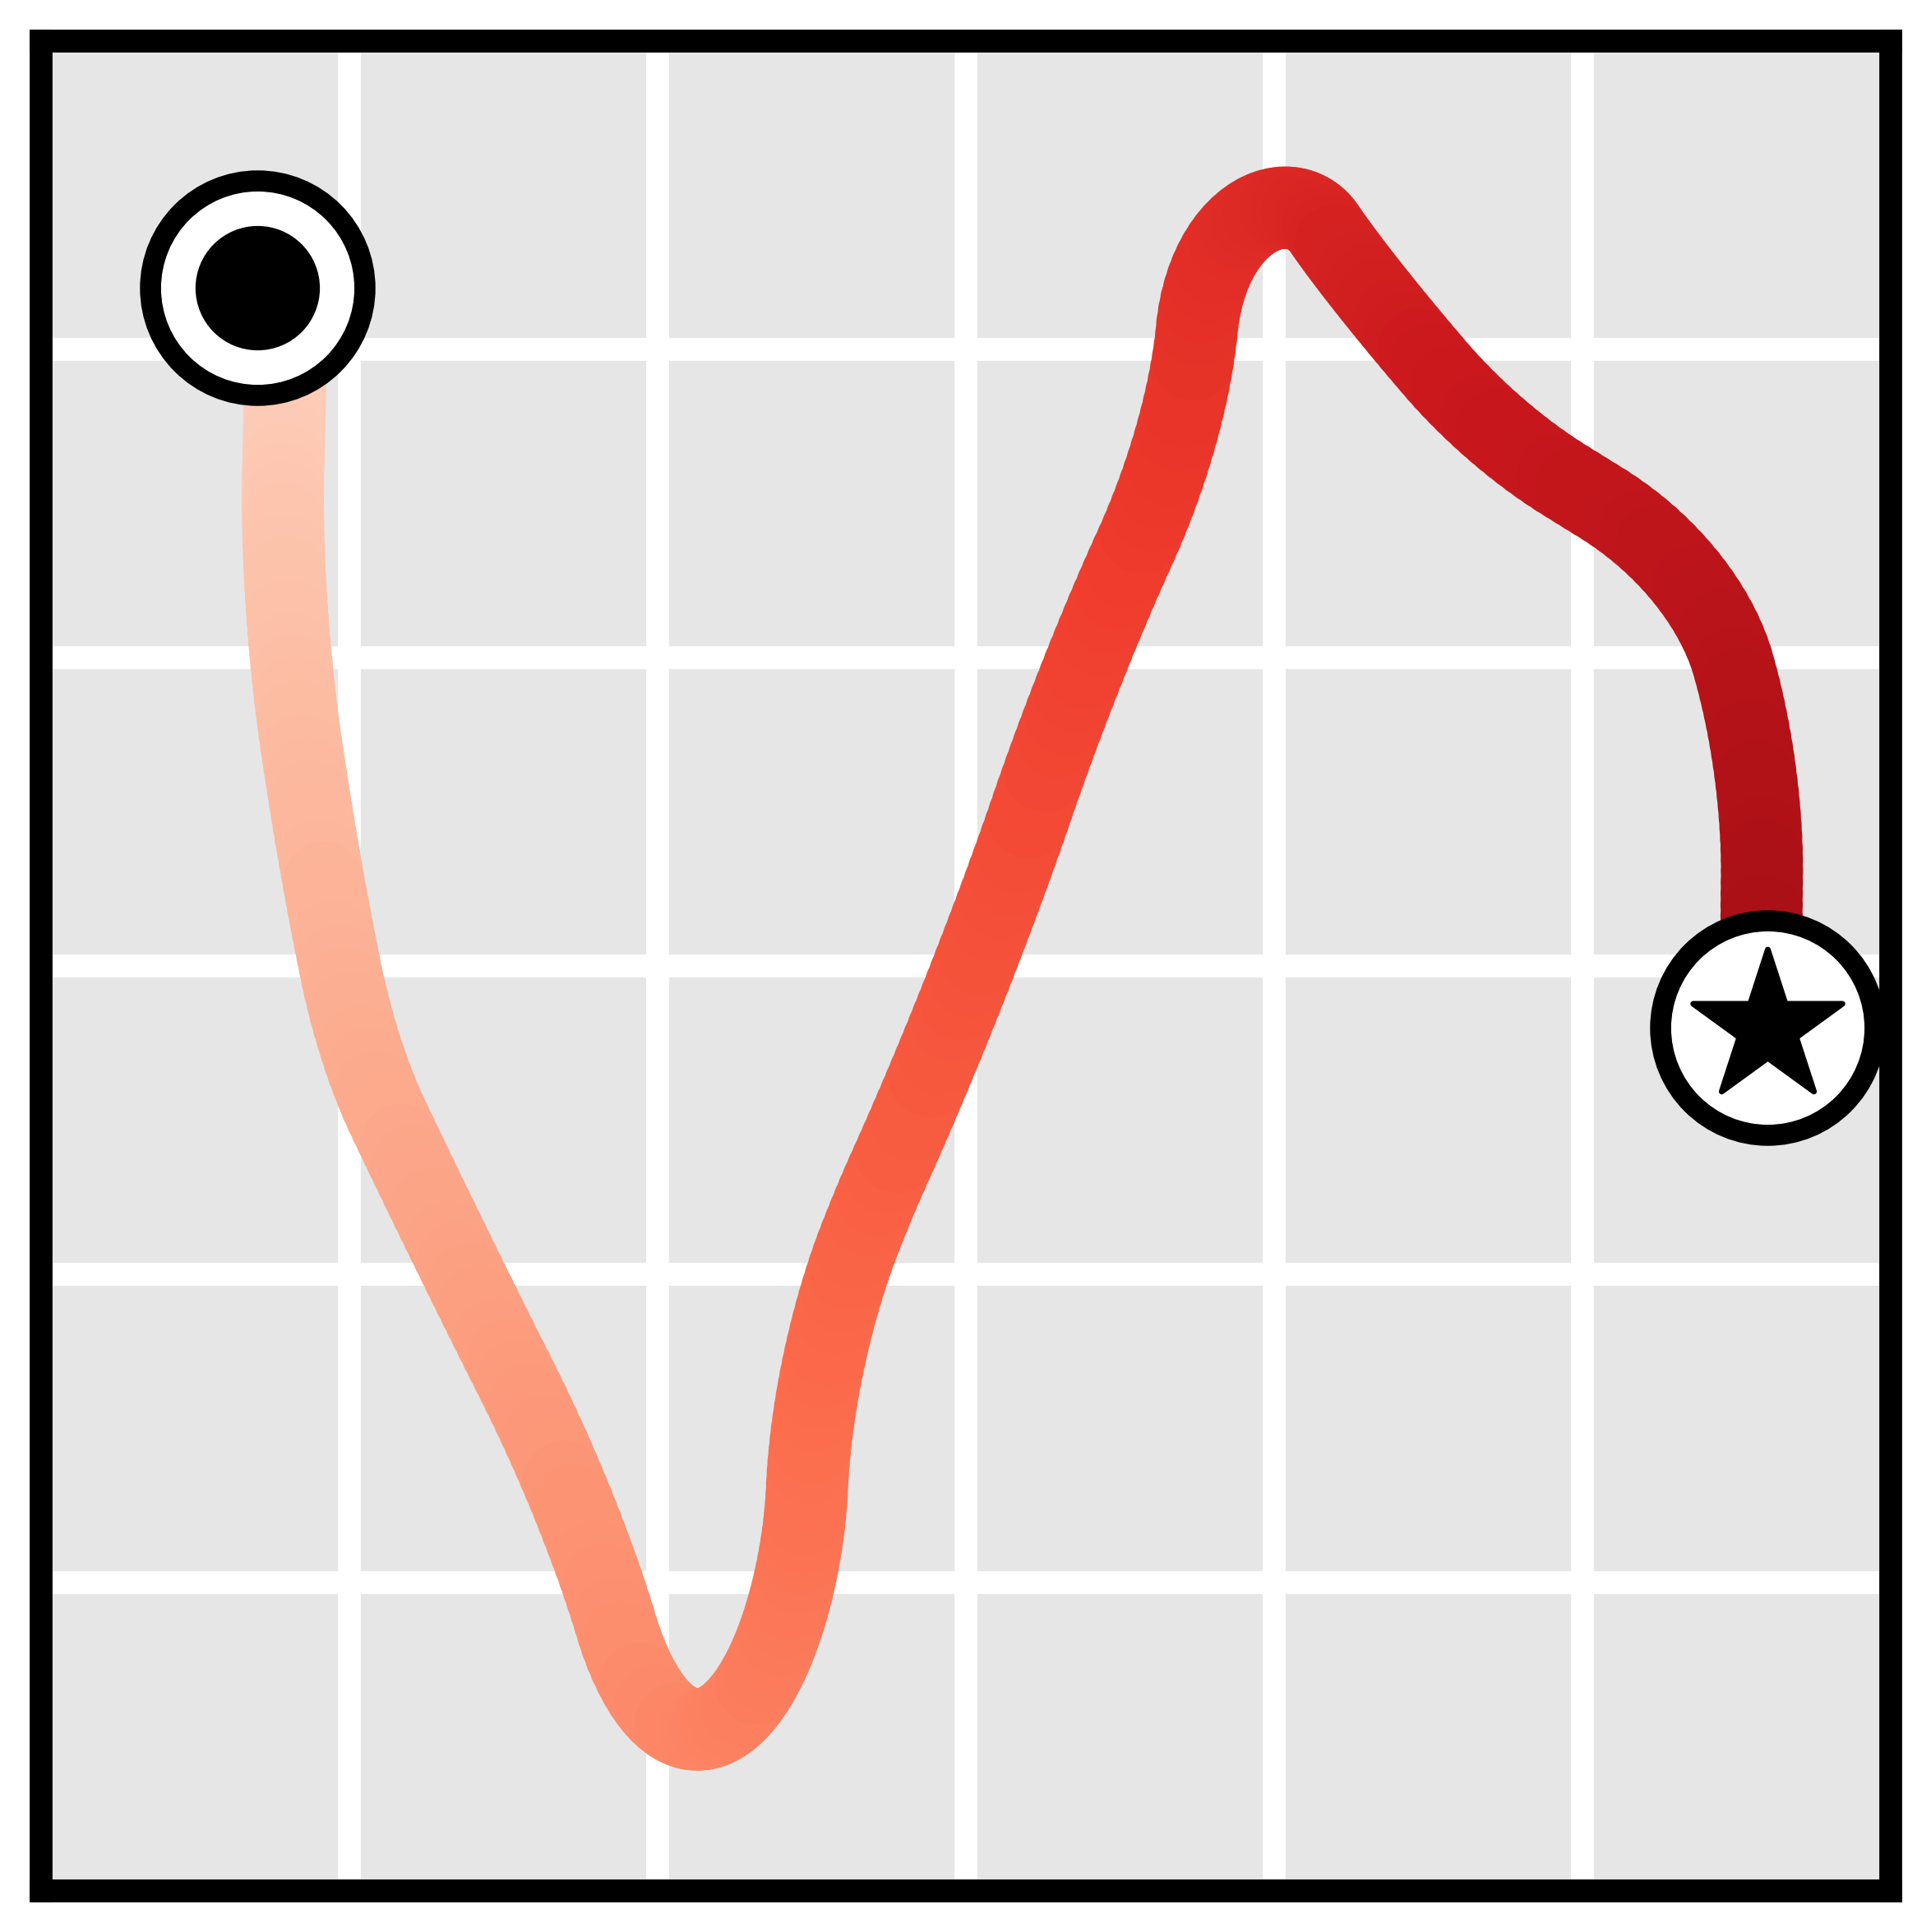
\includegraphics[width=2.5cm]{images/properties/reward_plan.png} \\
    \vspace{-.5cm}
    \begin{flushleft}
            \hspace{0.43cm} reward
            \hspace{0.0cm}
            \raisebox{.05cm}{$-$}
            \raisebox{.0cm}{
\includegraphics[height=1cm,angle=90]{images/properties/reward_colorbar.png}}
            \raisebox{.05cm}{$+$}
            \hspace{0.6cm} plan \\
    \end{flushleft}
\end{minipage}
\caption{
    % \small
    \textbf{(Properties of diffusion planners)}
    \textbf{(a) Learned long-horizon planning:}
    \method{}'s learned planning procedure does not suffer from the myopic failure modes common to shooting algorithms and is able to plan over long horizons with sparse reward.
    \textbf{(b) Temporal compositionality:} Even though the model is not Markovian, it generates trajectories via iterated refinements to local consistency.
    As a result, it exhibits the types of generalization usually associated with Markovian models, with the ability to stitch together snippets of trajectories from the training data to generate novel plan.
    \textbf{(c) Variable-length plans:}
    Despite being a trajectory-level model, \method's planning horizon is not determined by its architecture.
    The horizon can be updated after training by changing the dimensionality of the input noise.
    \textbf{(d) Task compositionality:} \method{} can be composed with new reward functions to plan for tasks unseen during training.
    In all subfigures,
    \protect{\raisebox{-.05cm}{
\includegraphics[height=.35cm]{images/maze2d/mark_start_crop.png}}}
    denotes a starting state and
    \protect{\raisebox{-.05cm}{
\includegraphics[height=.35cm]{images/maze2d/mark_goal_crop.png}}}
    denotes a goal state.
}
% \vspace{-.1cm}
\label{fig:properties}
% \vspace{-10pt}
\end{figure*}

\subsection{Reinforcement Learning as Guided Sampling}
\label{sec:guided}

In order to solve reinforcement learning problems with \method, we must introduce a notion of reward.
We appeal to the control-as-inference graphical model \citep{levine2018reinforcement} to do so.
Let $\mathcal{O}_{t}$ be a binary random variable denoting the optimality of timestep $t$ of a trajectory, with ${p(\mathcal{O}_t=1) = \exp(r(\st, \at))}$. We can sample from the set of optimal trajectories by setting ${h(\btau{}) = p(\mathcal{O}_{1:T} \mid \btau{})}$ in Equation~\ref{eq:perturbed}:
% \vspace{-.1cm}
\[
\tilde{p}_\theta(\btau{}) = p(\btau{} \mid \mathcal{O}_{1:T}=1) \propto p(\btau{}) p(\mathcal{O}_{1:T}=1 \mid \btau{}).
\]
% \vspace{-.7cm}

We have exchanged the reinforcement learning problem for one of \emph{conditional sampling}.
Thankfully, there has been much prior work on conditional sampling with diffusion models.
While it is intractable to sample from this distribution exactly, when $p(\mathcal{O}_{1:T} \mid \btau{i})$ is sufficiently smooth, the reverse diffusion process transitions can be approximated as Gaussian \citep{sohldickstein2015nonequilibrium}:
\begin{equation}
\label{eq:guided}
p_\theta(\btau{i-1} \mid \btau{i}, \opt_{1:T}) \approx \mathcal{N}(\btau{i-1}; \mu + \Sigma g, \Sigma)
\end{equation}

where $\mu, \Sigma$ are the parameters of the original reverse process transition $p_\theta(\btau{i-1} \mid \btau{i})$ and
% \vspace{0cm}
\begin{align*}
g &= \nabla_{\btau{}} \log p(\opt_{1:T} \mid \btau{}) |_{\btau{} = \mu} \\
&= \sum_{t=0}^{T} \nabla_{\st,\at} r(\st, \at) |_{(\st,\at)=\mu_t}
= \nabla \mathcal{J}(\mu).
\end{align*}
\vspace{-.45cm}

This relation provides a straightforward translation between classifier-guided sampling, used to generate class-conditional images \citep{dhariwal2021diffusion}, and the reinforcement learning problem setting.
We first train a diffusion model $p_\theta(\btau{})$ on the states and actions of all available trajectory data.
We then train a separate model $\mathcal{J}_\phi$ to predict the cumulative rewards of trajectory samples $\btau{i}$.
The gradients of $\mathcal{J}_\phi$ are used to guide the trajectory sampling procedure by modifying the means $\mu$ of the reverse process according to Equation~\ref{eq:guided}.
The first action of a sampled trajectory ${\btau{} \sim p(\btau{} \mid \mathcal{O}_{1:T}=1)}$ may be executed in the environment, after which the planning procedure begins again in a standard receding-horizon control loop.
Pseudocode for the guided planning method is given in Algorithm~\ref{alg:rl}.

\subsection{Goal-Conditioned RL as Inpainting}
\label{sec:inpainting}

Some planning problems are more naturally posed as constraint satisfaction than reward maximization.
In these settings, the objective is to produce any feasible trajectory that satisfies a set of constraints, such as terminating at a goal location.
Appealing to the two-dimensional array representation of trajectories described by Equation~\ref{eq:trajectory_array}, this setting can be translated into an \emph{inpainting problem}, in which state and action constraints act analogously to observed pixels in an image \citep{sohldickstein2015nonequilibrium}.
All unobserved locations in the array must be filled in by the diffusion model in a manner consistent with the observed constraints.

The perturbation function required for this task is a Dirac delta for observed values and constant elsewhere.
Concretely, if $\mathbf{c}_t$ is state constraint at timestep $t$, then
% \vspace{-.05cm}
\[
    h(\btau{}) = \delta_{\mathbf{c}_t}(\bs_0,\ba_0,\ldots,\bs_T,\ba_T) =
\begin{cases}
    +\infty      & \text{if } \mathbf{c}_t = \st\\
    ~~~~~0      & \text{otherwise}
\end{cases}
\]
% \vspace{-.05cm} \\
The definition for action constraints is identical.
In practice, this may be implemented by sampling from the unperturbed reverse process ${\btau{i-1} \sim p_\theta(\btau{i-1} \mid \btau{i})}$ and replacing the sampled values with conditioning values $\mathbf{c}_t$ after all diffusion timesteps $i \in \{0, 1, \ldots, N\}$.

Even reward maximization problems require conditioning-by-inpainting because all sampled trajectories should begin at the current state.
This conditioning is described by line 10 in Algorithm~\ref{alg:rl}.
